\documentclass{iitthesis}

%   \documentclass[draft]{iitthesis}

%\usepackage[dvips]{graphicx}    % This package is used for Figures
\usepackage{graphicx}    % This package is used for Figures
\usepackage{epstopdf}
\usepackage{placeins}
%\usepackage{rotating}           % This package is used for landscape mode.
\usepackage{epsfig}
\usepackage{subfigure}          % These two packages, epsfig and subfigure, are used for creating subplots.
\usepackage{mathtools}          % used for equations
\usepackage{listing}
\usepackage{xcolor}
\usepackage[final]{mcode}
% Packages are explained in the Help document.


\begin{document}
%%fakesection{TITLES AND INDEXES)
%%% Declarations for Title Page %%%
\title{Energy savings for UAV flight in unsteady gusting conditions \\
through trajectory optimization }
\author{Lou Grimaud}
\degree{Master of Science}
\dept{Mechanical, Materials, and Aerospace Engineering}
\date{July 2014}
%\copyrightnoticetrue      % crate copyright page or not
\maketitle                % create title and copyright pages


\prelimpages         % Settings of preliminary pages are done with \prelimpages command


%%%  Acknowledgement %%%
\begin{acknowledgement}     % acknowledgement environment, this is optional
  \par I would like to thank my advisor Dr Williams for his guidance and trust.
  The results presented in this dissertation would have not been obtained without the help of my lab-mates, Xuanhong An, Simeon Iliev and Jeremy Weirich.

\end{acknowledgement}


% Table of Contents
\tableofcontents
\clearpage

% List of Tables
%\listoftables
%
%\clearpage

%List of Figures
\listoffigures

\clearpage

%List of Symbols(optional)

\listofsymbols


\SymbolDefinition{$C_l$}{Lift coefficient}
\SymbolDefinition{$C_d$}{Drag coefficient}
\SymbolDefinition{$y_i$}{Vector of position and velocities at point $i$}
\SymbolDefinition{$W_a$}{Non-dimensional gust amplitude}
\SymbolDefinition{$T_c$}{Vehicle time scale ($=\frac{V_cr}{g}$)}
\SymbolDefinition{$T_g$}{Non-dimensional gust duration}
\SymbolDefinition{$T$}{Non-dimensional vehicle time ($=\frac{t}{T_c}$)}
\SymbolDefinition{$V^*$}{Vehicle cruse speed}
\SymbolDefinition{$C_l^*, C_d^*$}{Lift and drag coefficients at the optimal lift to drag ratio}
\SymbolDefinition{$G$}{lift to drag ratio}
\SymbolDefinition{$G^*$}{optimal (maximal) lift to drag ratio}
\SymbolDefinition{$Q$}{Non-dimensional dynamic pressure}
\SymbolDefinition{$X, Z, U, W$}{Non-dimensional positions and velocities}
\SymbolDefinition{$v$}{Relative wind velocity to the vehicle}
\SymbolDefinition{$L', D'$}{Lift and drag forces}
\SymbolDefinition{$V^*$}{Optimal glide speed}
\SymbolDefinition{$\gamma$}{Angle of the vehicle trajectory to the horizon}
\SymbolDefinition{$U_g, W_g$}{Non-dimensional horizontal and vertical gust velocity components}
\SymbolDefinition{$u$}{Free stream velocity}
\SymbolDefinition{$c$}{Airfoil chord}
\SymbolDefinition{$t^+$}{Airfoil time scale ($=\frac{u}{c}$)}
\SymbolDefinition{$k$}{Non-dimesional reduced frequency ($=\pi c \frac{f}{u}$)}
\SymbolDefinition{$x$}{State vector used for the optimizatiion}
\SymbolDefinition{$C_l^{qs}, C_d^{qs}$}{Quasi-steady lift and drag coefficients}
\SymbolDefinition{$x_0$}{State variable x value for quasi-steady cases}
%
\clearpage

%%% END OF INDEXES %%%
%%%%%%%%%%%%%%%%%%%%%%%%%%%%%%%%%%%%%%%%%%%%%%%%%%%%%%%%%%%%%%%%%%%%%%%%%%%%%%%%%%%%%%%

%%% Abstract %%%
\begin{abstract}           % abstract environment, this is optional
  \par The purpose of this thesis is to show how micro unmanned aerial vehicles can extract energy from natural wind gusts and how this energy extraction is affected by the effects of unsteady aerodynamics.

\par The trajectory of a small UAV flying through wind gusts is simulated with a two degrees of freedom model.
The non-dimensional model is set to include vertical and horizontal gusts of varying amplitudes and durations.
From this model an optimization routine is performed in order to obtain the minimum gust amplitude needed to get a neutral energy trajectory.
With these results, it is shown that neutral energy flight is possible through gusts speeds only 10 to 30\% of the flying speed of the aircraft .
Analysis of the results shows that the lift coefficient has to be changed very rapidly in order to perform these maneuvers in short duration gusts. 
Moreover high lift values are often required. 

\par To achieve this kind of rapid changes in the lift and drag forces, fast variations of the angle of attack are needed.
The high lift values also requires high angles of attacks that are likely to cause separation of the flow over the airfoil.
These fast variations at high angle of attack are shown to cause unsteady non linear aerodynamic responses.
Traditional CFD simulations are far too computationally expensive to be implemented into the optimization routine.
To solve this issue a low order model based on a paper by Goman and Khrabrov \cite{GK} is developed and validated against experimental results.
This model produces accurate predictions of the lift and drag coefficients for a wide range of angle of attack and for different type of pitch inputs.

\par With this light model the influence of the unsteady aerodynamics on the energy extraction problem are highlighted.
The main difference with quasi-steady aerodynamics model was found to be for gusts at a reduced frequency faster than k of 0.07.
Around these values the potential performances are improved by introducing the unsteady model.
The trajectories obtained include more violent changes in angle of attacks in order to take full advantages of the unsteady effects.



  %you need a separate abstract.tex file to include it.
\end{abstract}


\textpages     % Settings of text-pages are done with \textpages command

% Chapters are created with \Chapter{title} command
\Chapter{INTRODUCTION}

\Section{Motivations} \label{subsec:dynsoar}

\Subsection{Trajectory optimization through wind gusts}
The main challenge for electric small size unmanned aerial vehicle is the autonomy.
Battery energy density is limited and can rapidly become a important part of the weight of vehicle.
Since most of the energy is used by the electric engine for propulsion, optimizing the control laws and trajectory could have a dramatic effect on endurance. 
With the progress in autonomous control software successful attempt have been made by Allen \cite{flight_test_soaring_NASA} and Edwards \cite{flight_test_soaring_NCU} to extract energy from natural updraft.
These experiments have shown that an UAV can take advantage of localized vertical winds naturally produced by thermal convection.

\par However, within an urban environment, such as the one mini and micro-UAV are made for, the gust's profile is vastly different. 
Wind blowing through an group of building produce turbulent conditions with both vertical and horizontal vortexes.
These turbulences can reach speed representing a significant portion of micro-UAV's glide speed. 
In flow fields such as this the gusts encountered are both faster and arguably more complex than the ones due to thermal convection.

\par The lack of low order models for the unsteady effects meant that all of the studies on trajectory optimization seemed to have focused on quasi-steady models to compute the aerodynamic forces.
More computationally expensive model traditionally used for CFD are too unpractical considering the thousands of functions evaluations needed for such algorithm.
To solve this problem a low order model capturing the unsteady behavior of the flow over the aircraft is needed.
Additionally this model needs to be able to handle flow separation and airfoil stalling since the maneuvers required for energy extraction can be relatively violent and often involve high angle of attack.


\Subsection{Pitching airfoil model}
The difficulty is that the lift and drag behavior in such condition is time dependent and non-linear.
As such finite elements methods are often the only solution to get a good simulation of the lift and drag.
Such solution are useful since they provide a lot of information about the flow flied itself, but the computation time required to get the lift and drag out of them is several order of magnitude too long.

\par Another solution explored by Brunton \cite{brunton2008unsteady} is to perform linear approximations of the lift and drag behavior at different angles of attack.
These linear models can then be patched together to include the non-linear behaviors.
The appeal of this method is that the individual linear models can be easily analyzed using classical LTI system theory.
It is however still fairly complicated and requires an extensive experimental study to identify the system at each set angle of attack.

\par The model developed by Goman and Khrabrov allows for a low order model non linear model to capture the features of the lift coefficient over a very wide range of angle of attack as well as for any arbitrary pitch profile.
One quasi-steady map of the lift and two time constants are all that is needed to get the full model.
So far it seems that the use of this model has been limited to the lift coefficient predictions however for the trajectory optimization the drag coefficient is also needed.

\Section{Previous investigations/literature review}

\par As explained in the previous part \ref{subsec:dynsoar}, the bulk part of the research on trajectory optimization for small flying vehicle has been focused on either natural convection such as the one glider pilots and some birds of prey take advantage of in plains, or wind gradients such the ones found close to the surface of the ocean.
The later are often exploited by seabird such as albatrosses.

\par Lissaman \cite{lissaman2005wind} has conducted a study for 3D trajectories in differently shaped wind gradients close to the ground.
His optimization is performed on a non-dimensional set of equation that has been reused in this study.
He also uses different kind of profiles for the wind gradient in order to represent more accurately real wind gradients.


\Chapter{Energy extraction optimization} \label{ch:Eni_extraction}

\Section{2 DoF model}

\Subsection{Non-dimensional equations of motion}
The model chosen for this simulation is a simple two degree of freedom, two dimension, point mass model. 
The aircraft is assumed to be a glider to simplify the optimization routine. 
With such assumption the equations of motion in the ground reference frame is :

\begin{equation}
\begin{array}[c]{c}
  \ddot{x}= -L' \cdot sin(\gamma) + D' \cdot cos(\gamma) \\ 
  \ddot{z}= L' \cdot cos(\gamma) - D' \cdot sin(\gamma) - m \cdot g
\end{array}
\label{eqn:eqm}
\end{equation}

% should I include a figure with the reference frame, and angle definition?

\par The lift and drag are defined are: 

\begin{equation}
\begin{array}[c]{c}
  L'= \frac{1}{2} \rho v^2 C_l \\ 
  D'= \frac{1}{2} \rho v^2 C_d 
\end{array}
\label{eqn:Cl_def}
\end{equation}

\par With $v$ being the relative wind for the vehicle.
% do I need to include this kind basic stuff?

\par Since this simulation is mainly concerned with Newtonian physics (rather than fluid phenomenons) the usual fluid dynamics non-dimensional variables make little sense.
Here the equations are normalized by the optimal glide speed and $g$, the gravitational acceleration.
This is more representative of the performances of the aircraft.

\par Following Lissaman's \cite{lissaman2005wind} implementation of the equation of motion we define $V^*$ the optimal glide speed for the aircraft. 
This speed is achieved at the optimal lift to drag ratio of the aircraft.
With $C_l^*$ and $C_d^*$ the angle of attack for the maximum lift to drag ratio and $\gamma$ the pitch angle with respect to the horizon the optimal glide speed is:

\begin{equation}
\begin{array}[c]{c}
  \gamma^*= - atan(\frac{C_l^*}{C_d^*}) \\
  V^* = \sqrt{\frac{2mg}{\rho S (C_l^* cos(\gamma^*) - C_d^* sin(\gamma^*)}}
\end{array}
\label{eqn:glide_speed}
\end{equation}

\par From we define $U$ and $W$ the non dimensional horizontal and vertical speed in the inertial reference frame.

\begin{equation}
\begin{array}[c]{c}
  U = \frac{\dot{x}}{V^*} \\
  V= \frac{\dot{z}}{V^*}
\end{array}
\label{eqn:non_dim_speed}
\end{equation}

The time is normalized by $g / V^*$.

\par Since the speed is seen as a fraction of the optimal glide speed it makes sens to also normalize the lift and drag coefficients by their corresponding values at the optimal lift to drag ratio.

\begin{equation}
\begin{array}[c]{c}
  L= \frac{C_l}{C_l^*} \\
  D= \frac{C_d}{C_d^*} 
\end{array}
\label{eqn:non_dim_coef}
\end{equation}

\par Finally we introduce Q the dynamic pressure as:

\begin{equation}
Q = \frac{L'}{MgL} = \frac{\frac{1}{2} \rho V^2 C_l C_l^* }{Mg}
\label{eqn:dynamic_pressure}
\end{equation}

\par From there the equation of motion \ref{eqn:eqm} can be expressed as:

\begin{equation}
\begin{array}[c]{c}
  \frac{dU}{dT}= -LQ \cdot sin(\gamma) + DQ \cdot cos(\gamma) \\ 
  \frac{dW}{dT}= LQ \cdot cos(\gamma) - DQ \cdot sin(\gamma) - 1
\end{array}
\label{eqn:non_dim_eqm}
\end{equation}

With 

\begin{equation}
\gamma = -atan(\frac{W-W_g}{U-U_g})
\label{eqn:gamma_def}
\end{equation}

$W_g$ and $U_g$ are the vertical and horizontal wind speeds in the inertial reference frame.

\par Finally the remaining thing to consider is $Q$ the dynamic pressure. If we define the speed of the wind gust as $W_g$ and $U_g$ we can express:

\begin{equation}
Q = V^2 = (W-W_g)^2 + (U-U_g)^2
\label{eqn:q_def}
\end{equation}

\par With these definitions we have the basic formulation of our non-dimensional equation of motions, normalized by the performances at the optimal glide trajectory in a calm environment.

\Subsection{Lift and drag models}
The normalized equation of motion \ref{eqn:non_dim_eqm} are not accounting for the fluid dynamic part of the flight.
The most important factor for glide performance is the lift to drag ratio. 
In his paper, Lissaman \cite{Lissaman2007neutral} is using a relatively simple quadratic model for the relationship between lift and drag:

\begin{equation}
D=\frac{Q}{2G}(1+L^2)
\label{eqn:Lissaman_G}
\end{equation}

%[CHECK THIS EQUATION !!!!!]

\par This simple model work relatively well for simple airfoil but is inadequate for more complex shapes.
Moreover it fails to properly account for the effects of flow separation at high angle of attacks.
Finally this model is only valid for the quasi-steady flow conditions.

\par Since the unsteady model developed in chapter \ref{Ch:gkmodel} is based on experimental results for a NACA0009 airfoil, we will use simplified versions of the lift and drag characteristics of this airfoil.

\begin{figure}[ht]
\begin{center}
  \scalebox{0.8}
  {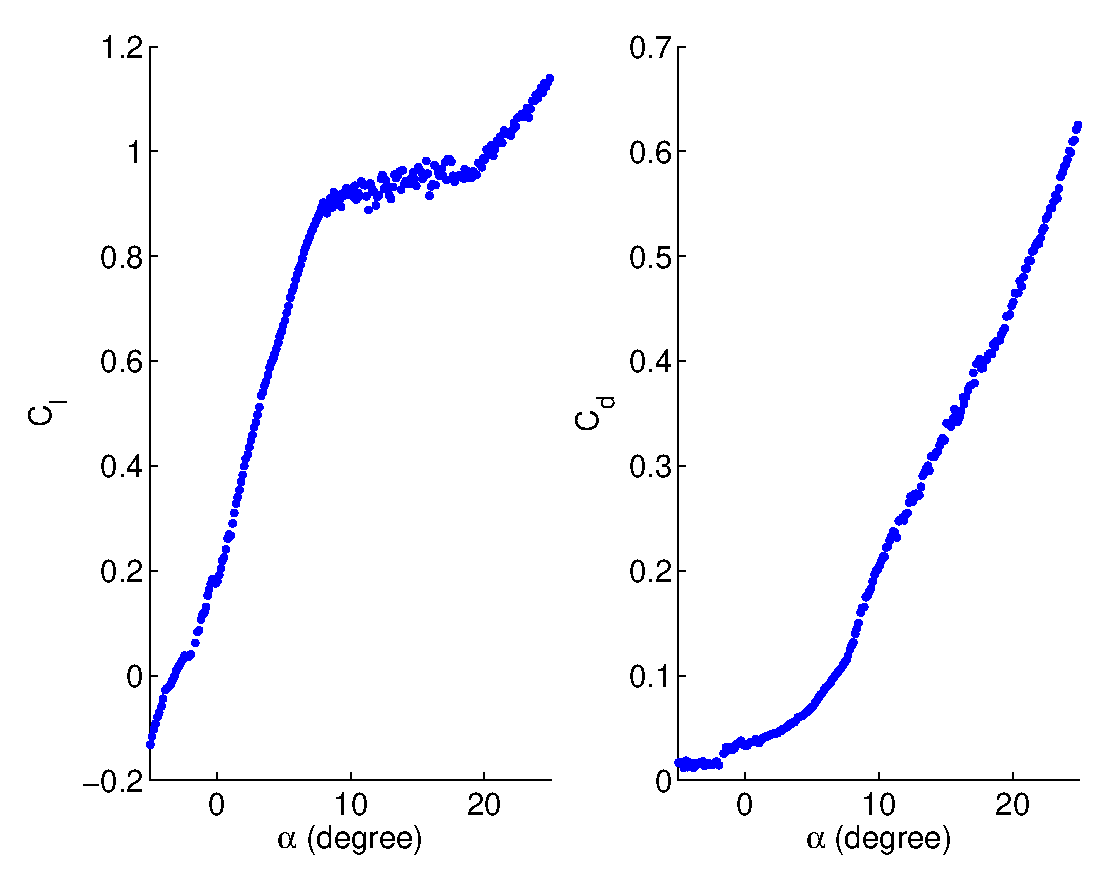
\includegraphics{./Figures/NACA0009_steady_map_Cl_Cd.eps}} 
\end{center}
\caption{Lift and drag characteristics of the NACA0009}
\end{figure}


\begin{figure}[ht]
\begin{center}
%    \scalebox{0.8}
%   {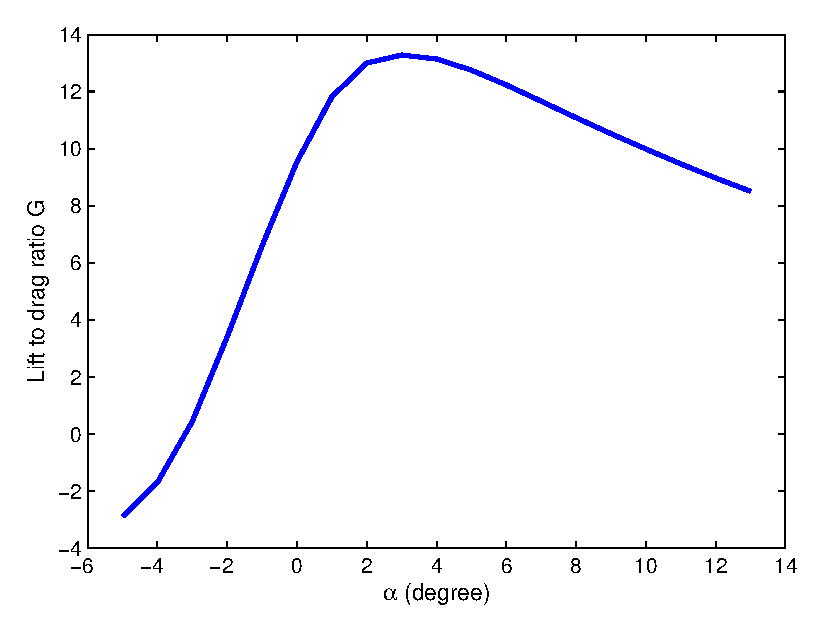
\includegraphics{./Figures/lift_to_drag_UAV.eps}}
\end{center}
\caption{Lift to drag ratio for the NACA0009}
\end{figure}

\par This results, while being arguably more realistic than a simple quadratic approach, are still only considering quasi-steady change in the angle of attack.
This limitation will be discussed more in depth in the result discussion section \ref{sec:results_QS}.

\Subsection{Wind profiles}
Most of the studies done on dynamic soaring has either been done with vertical wind gusts or thermal updraft, or horizontal wind gradient foxed in time.
In this optimization procedure we chose to consider three different wind profiles made out of first order sinusoidal gusts.

\par Our first gust profile is a simple vertical gust.

\begin{equation}
\begin{array}[c]{c}
  W_g = W_a \cdot sin(2\pi T) \\
  U_g = 0 
\end{array}
\label{eqn:vertical_gust_definition}
\end{equation}

\par Similarly the horizontal gust is defined as:

\begin{equation}
\begin{array}[c]{c}
  W_g = 0 \\
  U_g = W_a \cdot cos(2 \pi T)
\end{array}
\label{eqn:horizontal_gust_definition}
\end{equation}

\par Finally a more complex combined gust is defined.
This gust profile is the sum of the two previously defined gusts.
Moreover we introduce $\phi$, a phase difference between the two component of the gust. 

\begin{equation}
\begin{array}[c]{c}
  W_g = W_a \cdot sin(2\pi T) \\
  U_g = W_a \cdot cos(2 \pi T + \phi)
\end{array}
\label{eqn:combined_gust_definition}
\end{equation}

\Section{Optimization process, cost function and constraints}

\Subsection{General consideration on optimization}
% Get some stuff from the MM544 class
The general principle for the optimization routines resides in defining a so called ``cost function'' that will represent a quantity we want to minimize.
While the algorithm tries to minimize this scalar, a set of constraints have to be respected. 
These constraints can represent physical limitations or specific requirements related to the system at hand.
The cost and constraints are expressed as functions of a set of system state variables.
The state variables can represent temporal or spatial values.
The optimization is performed in a sequential fashion where different algorithm are used to step from one set of values for the state variables to another. 

\par Optimization routines are divided into two families. 

\par The first method is called the gradient method, it requires a good knowledge of the physics behind the problem.
The cost function as well as the constraints have to be explicitly defined.
In this method the gradient of the cost function and the constraints is used to determine the direction of the next step in the optimization.
Different algorithm are used to chose the step size, and sometime the direction of the previous step can influence the current step.
The gradients for either the cost function or the constraints do not have to be explicitly defined as modern optimization routines, such as the one included in Matlab, can perform numerical gradient estimation.
However inputting an user defined gradient into the routine will significantly speed up the overall process.

\par The second method is using the so called ``evolutionary algorithms''. 
This method relies a lot less on knowing the underlying physical phenomenon.
Its basic principle is a ``try and see'' process.
Random changes are performed on the state variables and their effects on the cost function are assessed.
The best steps are selected as a starting point for the next generation.
While with this method each step is a less computation intensive than with the previous method, the number of steps is a lot higher.

\par The first method has been used in this optimization as it provides more insight on the physics behind the problem.
However it should be noted that the resulting ``optimal'' point is usually only assured to be \emph{a local} minimum of the cost function.
Several different starting states should be tested to ensure that the optimization converges toward a reasonable minimum.



\Subsection{Cost function}
Our problem here consists in optimizing the trajectory in a gusting environment to minimize energy lose.
The most obvious cost function would be something like

\begin{equation}
  - \frac{1}{2}m{V(T_f)}^2 - gX(T_f)
  \label{eqn:eni_cost_fun}
\end{equation}

Which would be equivalent to maximizing the total energy at the end of the gust.
However after testing this has shown to leave to much freedom to the algorithm. 
As a result the local minimum found are the result of trajectories such as very steep dives, clearly far from the optimum.

\par Once again we refer to the Lissaman paper \cite{Lissaman2007neutral} and chose, instead of minimizing energy loss for a given gust condition, to find the minimum gust amplitude to satisfy an energy neutral trajectory over the gust period.
This means that the cost function is the wind gust amplitude, which will have to be added to the state vector in order to be explicit, and that the neutral energy trajectory will have to be added to the constraints

\Subsection{State vector and constraints formulation}
In our case a gust cycle of duration $T_f$ is divided into $N$ discrete instants $T_i$ (usually between 31 and 101).
At each of these points we need to know the state of the vehicle.
Since we are considering a two degree of freedom model the two positions $X$, $Z$ and speed $U$, $W$ variables are the most simple choices.
However this is not enough to describe the system completely, we also need to know what our input is going to be, in this case the lift available and where on the lift vs drag curve we are.
Theres is two possible choices for this.
If you consider only the quasi steady part, the angle of attack $\alpha$ seems obvious.
However since the drag is a function of the lift (the inverse is not true), it is possible to use only the $L$ to define our point on the lift to drag curve.
This allows us to use one less variable.

\par With this five variables defined at each considered time points the state and input vector look like:

\begin{equation}
  x= 
  \begin{bmatrix}
    \cdots \\
    X_i \\
    Z_i \\
    U_i \\
    W_i \\
    L_i \\
    \cdots \\
    W_a
  \end{bmatrix}
  \quad i \in [1,N]
  \label{eqn:big_vector}
\end{equation}

\par All this variables have to be constrained to achieve a realistic trajectory.
The first and most obvious constrain is done with the equation of motion \ref{eqn:non_dim_eqm}.
This equation has to be changed from a continuous differential equation to a discrete equation.
This is done by using the Simpson's 1/3rd rule as derived by Zhao \cite{zhao2004optimal}.

In order to satisfy the equations of motion we need to define the state variable at the time $T_i$:

\begin{equation}
  y_i= \begin{bmatrix}
    X_i \\
    Z_i \\
    U_i \\
    W_i 
  \end{bmatrix}
  \label{eqn:state_i}
\end{equation}

Then with $\dot{y_i}$ the derivative of the state variables, given by the equation of motion \ref{eqn:non_dim_eqm} and:

\begin{equation}
  \begin{array}[c]{c}
    y_m= \frac{1}{2}(y_k + Y_{k+1}) - \frac{1}{8}(\dot{y_{k+1}} - \dot{y_k})\delta t \\
    L_m=\frac{1}{2}(L_i + L_{i+1})
  \end{array}
  \label{eqn:simpson_middle}
\end{equation}

The condition to satisfy the equation of motion becomes

\begin{equation}
  0=y_{k+1} - y_k - \frac{1}{6}( \dot{y_k} + 4 \dot{y_m} + \dot{y_{k+1}})\delta t \quad \forall i \in [1,N-1]
  \label{eqn:simpson}
\end{equation}

\par Another constraint is on the neutral energy loop condition.
To account for that the initial and final $Z$ values are fixed at zero and the initial and final vertical and horizontal speeds are set to be equal.

\par Since we are looking at only one cycle, in order for it to be repeatable, we need to have a smooth transition from one to another.
This  means setting the derivative of the speed to be equal at the start and at the end of the cycle.

\begin{equation}
  \begin{array}[c]{c}
    W_2 - W_1 = W_N - W_{N-1} \\
    U_2 - U_1 = U_N - U_{N-1} 
  \end{array}
  \label{eqn:derivative_constraint}
\end{equation}

\par Finally the last set of constraint is on the physical limits of the aircraft.
Typically an aircraft flight envelope is limited by its maximum speed (depends on the dynamic pressure), its maximum load and its maximum lift (which determines the stalling speed).
Since our aircraft is will be flying around its optimal glide speed, over speeding isn't going to be an issue.
Moreover the drag increasing proportionally to the square of speed, high speeds will be avoided as much as possible by the optimization routine.
The limit on the load can conveniently be expressed as:

\begin{equation}
  L_i Q_i \leq g_max \quad \forall i \in [1,N]
  \label{eqn:load_constraint}
\end{equation}

With $g_max$ the maximum load in Gs.

% did I actually used that in my code? I think it wasn't necessary.

\par Finally the maximum lift condition can be expressed

\begin{equation}
  L_i \le \frac{C_l^{max}}{C_l^*} \quad \forall i \in [1,N]
  \label{eqn:lift_constraint}
\end{equation}

As it will be seen in section \ref{sec:results_QS} the value of $C_l^{max}$ has a profound impact on the performances of the UAV.

\par It is also sometime advisable to limit $\gamma$ in the $\pm 90^{\circ}$ range to prevent loops and backtracking.


\Subsection{Matlab optimization function}
Matlab offers several ways of doing optimization.
Since this scripting language allows for easy parallelization, it is relatively painless to implement your own optimization code.
However in most cases, ``classical'' optimization problems, such as weight reduction, topology optimization or mechanism design are reducible to a set of linear  equations and constraints.
In our case the equations of motions as well as the lift and drag properties are not linear at all, and trying to linearize this problem would make any solution meaningless.
For this reason a already existing optimization function has been chosen.

\par Since non linear optimizations like that are a computation intensive process dedicated tools have been developed to tackle the problem.
SNOP is one of these software and seems to be widely used.
Another tool appearing in the literature is a Fortran library called NPSOL.
Since our laboratory's language of predilection is Matlab, the optimization toolbox from MathWorks was used.

\par The optimization toolbox provides with a helpful function for non-linear optimization called \emph{fmincon()}.
This function needs an initial guest for the $x$ vector.
When using this function the initial guest has quite a big influence on the converging speed and on the local optimal solution found.
To account for that several educated guesses were made and tested for the different types of the wind profiles and gusts duration.
These guesses are refined as new results are obtained.


\Section{Results for quasi-steady aerodynamics} \label{sec:results_QS}

\Subsection{Typical trajectories}

\Subsection{Implementation validation}
The first step is to validate the code implemented here against previous results. 
Even if the lift and drag profiles are different from Lissaman's assumptions a similar case is optimized.
The gust duration is set to be $T_g=4 T$, for a purely vertical gust.
Since it is only a validation test the same lift and drag characteristics are used. Equation \ref{eqn:Lissaman_G} plugged into the equation of motion part of the code. An optimal lift to drag ratio of $G_{max}=20$ is chosen, as seen in the original Lissaman paper \cite{Lissaman2007neutral}.

\begin{figure}[ht]
  \begin{center}	
    \scalebox{0.8}
    {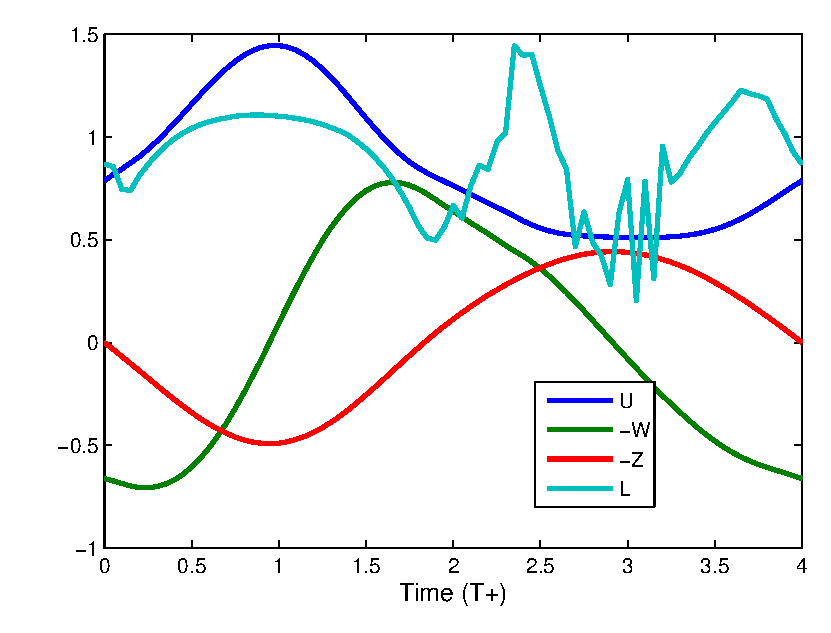
\includegraphics{./Figures/Windtype=1_Tg=4_Wg=0p129_quad_G=20.eps}}
  \end{center}
  \caption{Optimization results for a $4T$ long vertical gust}
  \label{fig:Validation_optimization}
\end{figure}

\FloatBarrier

Lissaman, with is optimal lift to drag ratio of 20 found a wind gust amplitude of $0.129$. 
Here the minimum required for neutral energy loop is $0.128$ (see figure \ref{fig:Validation_optimization}).
The shape of the state and control parameters curves are also consistent with the Lissaman results.

\par Similarly an optimization is performed for a purely horizontal wind gust.

\begin{figure}[h]
  \begin{center}
    \scalebox{0.8}
    {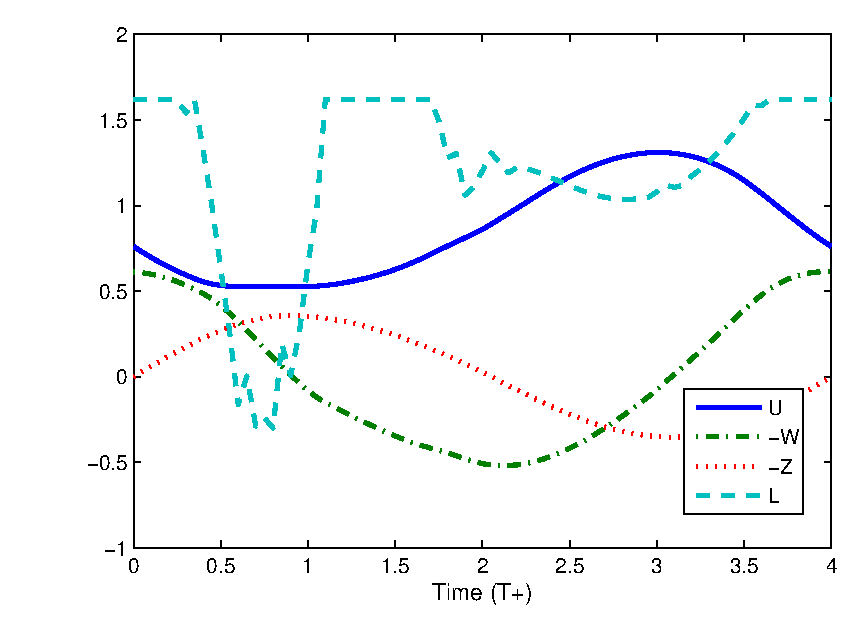
\includegraphics{./Figures/Windtype=2_Tg=4_Wg=0p246_quad_G=20.eps}}
  \end{center}
  \caption{$4T$ long horizontal gust for $G=20$, $W_a=0.246$}
  \label{fig:Horizontal_optimization}
\end{figure}

The resulting minimum wind amplitude is higher than for the vertical gust. 
However this shows that it is possible to take advantage of horizontal wind gusts to save energy if the performances are high enough.

\par Finally a combined horizontal and vertical gust is simulated.

\begin{figure}[h]
  \begin{center}
    \scalebox{0.8}
    {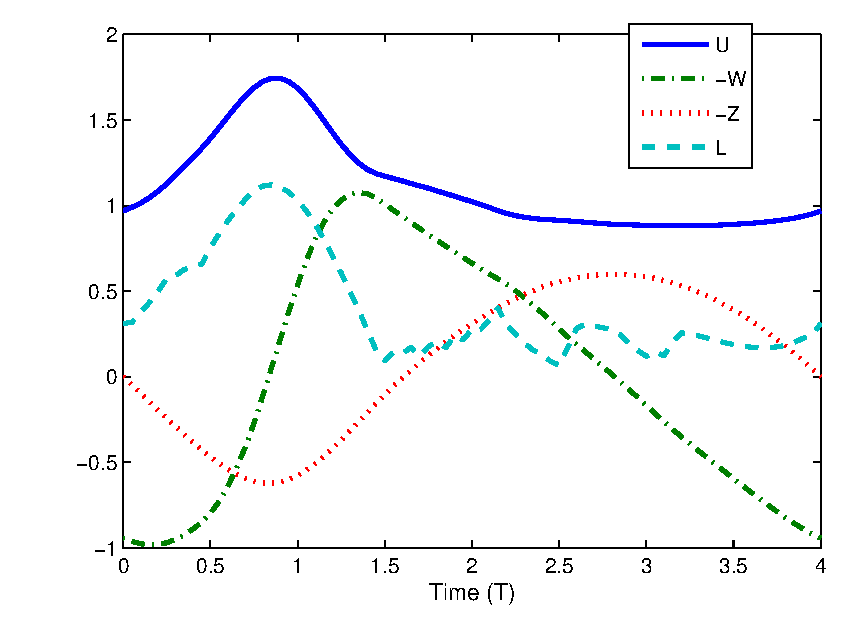
\includegraphics{./Figures/Windtype=3_Tg=4_Wg=0p232_quad_G=20.eps}}
  \end{center}
  \caption{$4T$ long combined gust for $G=20$, $W_a=0.232$}
  \label{fig:combined_optimization}
\end{figure}

Unsurprisingly the neutral energy loop trajectory exists also for this case.

\FloatBarrier

\Subsection{Typical results for the NACA0009 wing}

\par A similar batch of optimizations is done with the more realistic lift and drag profiles.
However since the lift to drag ration is lower than what Lissaman used in his model a higher gust amplitude is expected.

\begin{figure}
  \begin{center}
   \scalebox{0.8}
   {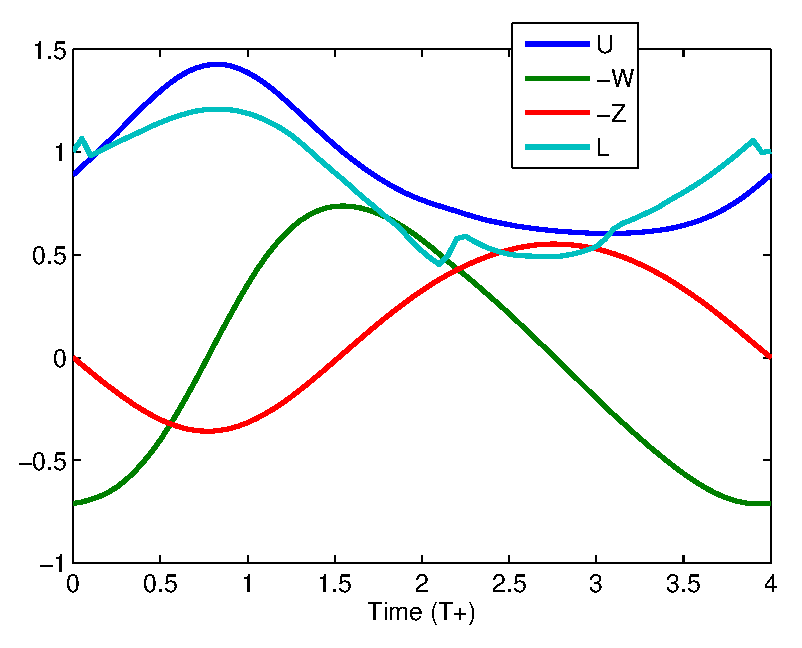
\includegraphics{./Figures/Windtype=1_Tg=4_Wg=0p205_UAV_alphamax=12.eps}}
  \end{center}
  \caption{$4T$ long vertical gust for UAV, $W_a=0.205$}
  \label{fig:vertical_optimization_UAV}
\end{figure}


\begin{figure}[h]
  \begin{center}
    \scalebox{0.8}
    {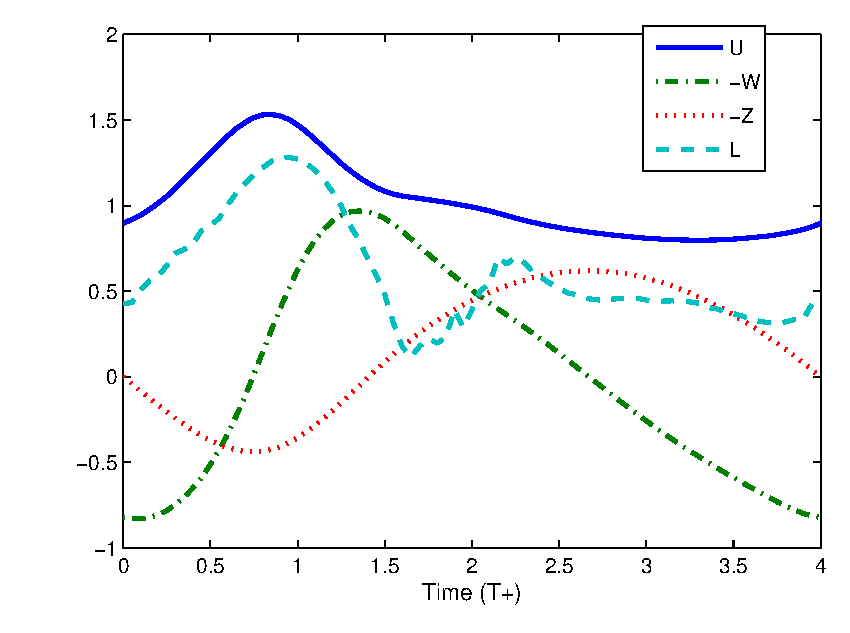
\includegraphics{./Figures/Windtype=3_Tg=4_Wg=0p387_UAV_alphamax=12.eps}}
  \end{center}
  \caption{$4T$ long combined gust for UAV, $W_a=0.387$}
  \label{fig:combined_optimization_UAV}
\end{figure}

As it can be seen on the figures \ref{fig:vertical_optimization_UAV} and \ref{fig:combined_optimization_UAV} the trajectories are similar in shape. However the gust amplitude needed to achieve neutral energy flight are a lot higher.
Such differences can be explained by looking at the maximum lift to drag ratio for both conceptual aircraft.
The quadratic drag profile used by Lissaman has a $G_{max}$ of 20.
The notional UAV used is closer to 14.

\FloatBarrier

\par With this kind of performances, a purely horizontal gust can't sustain a neutral energy loop.


\par To account for these differences a third batch of simulation is performed with by setting the $G_{max}$ parameter in the quadratic drag profile to 13.3.

\begin{figure}[ht]
  \begin{center}
    \scalebox{0.8}
    {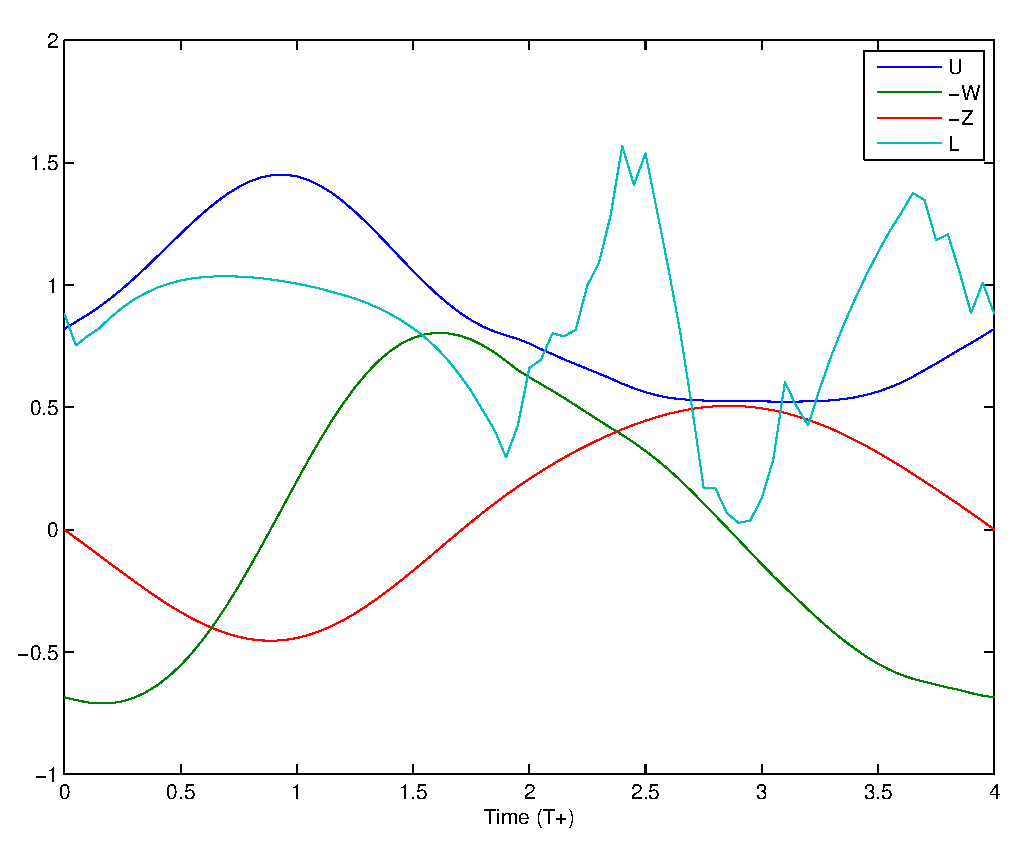
\includegraphics{./Figures/Windtype=1_Tg=4_Wg=0p194_quad_G=13.eps}}
  \end{center}
  \caption{$4T$ long vertical gust for $G=14$, $W_a=0.194$}
  \label{fig:vertical_optimization_UAV_modified}
\end{figure}


\begin{figure}[ht]
  \begin{center}
    \scalebox{0.8}
    {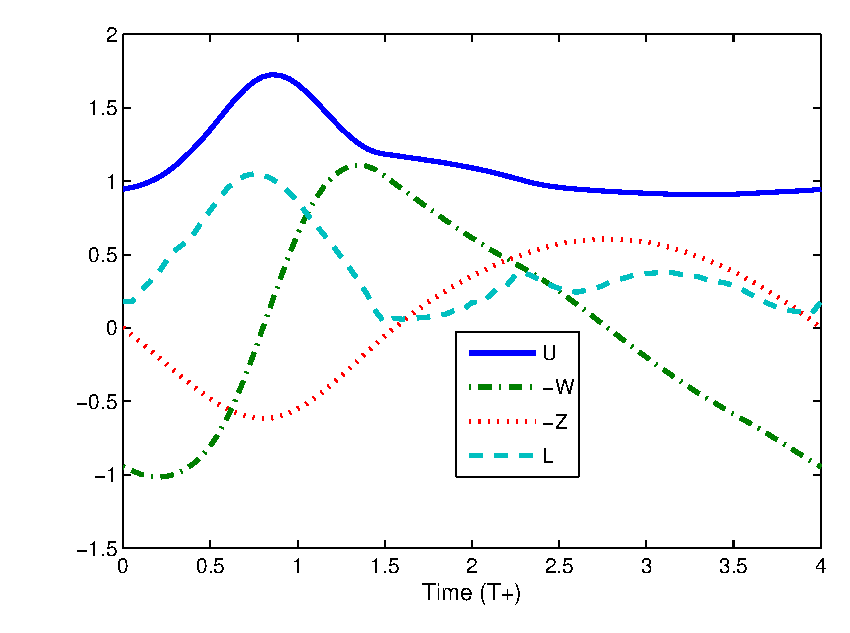
\includegraphics{./Figures/Windtype=3_Tg=4_Wg=0p360_quad_G=13.eps}}
  \end{center}
  \caption{$4T$ long combined gust for $G=14$, $W_a=0.360$}
  \label{fig:combined_optimization_UAV_modified}
\end{figure}

\par The results are similar.
Since the quadratic lift to drag profile isn't that different to the UAV one, the optimized gust amplitude is relatively close for both case.

\FloatBarrier

%\par Now that we have shown that for each type of trajectories the general behavior is the same, independently of the lift to drag ratio, it is interesting to compare at what time the energy was gained and at what rate it was changing.
%
%\par In the following figure the potential energy and kinetic energy are dissociated to highlight the actual effects of the altitude and speed gain.

% Do I want to make a trajectory/vector graph ??


\Subsection{Influence of the gust duration}
From our literature review it seems like most of the studies done on gusting winds has been conducted on gusts duration greater than $2T$.
Considering shorter gusts seems unreasonable of you only consider quasi steady aerodynamics, a $2T$ gust is about 2 seconds for vehicle flying 10 m/s.
However since the purpose this research is to extend the energy extraction envelope, such cases should be considered.

\begin{figure}[h!]
  \begin{center}
%    \scalebox{0.8}
%    {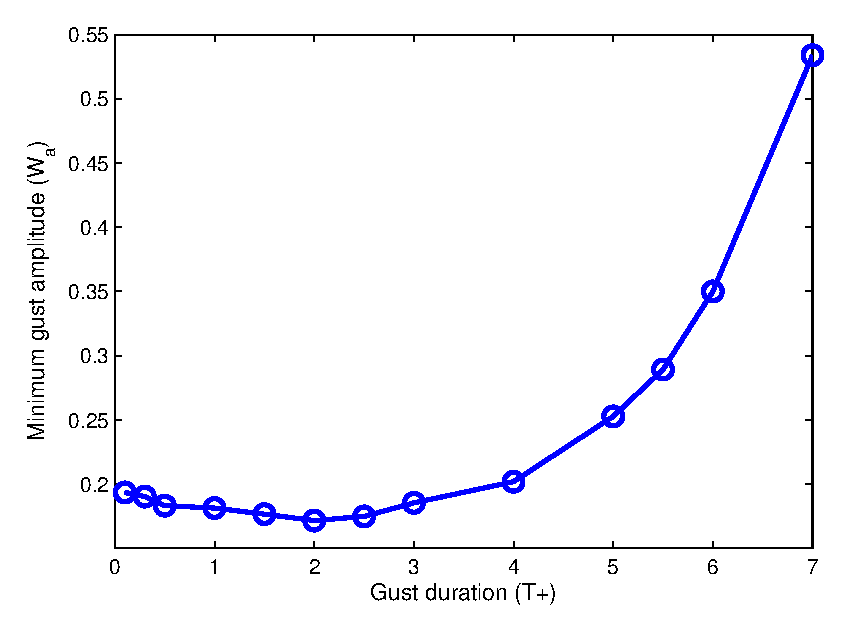
\includegraphics{./Figures/Vertical_gust_amplitude_vs_duration.eps}}
  \end{center}
  \caption{Influence of gust duration on the minimum gust amplitude for vertical gusts}
  \label{fig:vertical_amplitude_duration}
\end{figure}

\begin{figure}[h!]
  \begin{center}
%    \scalebox{0.8}
%    {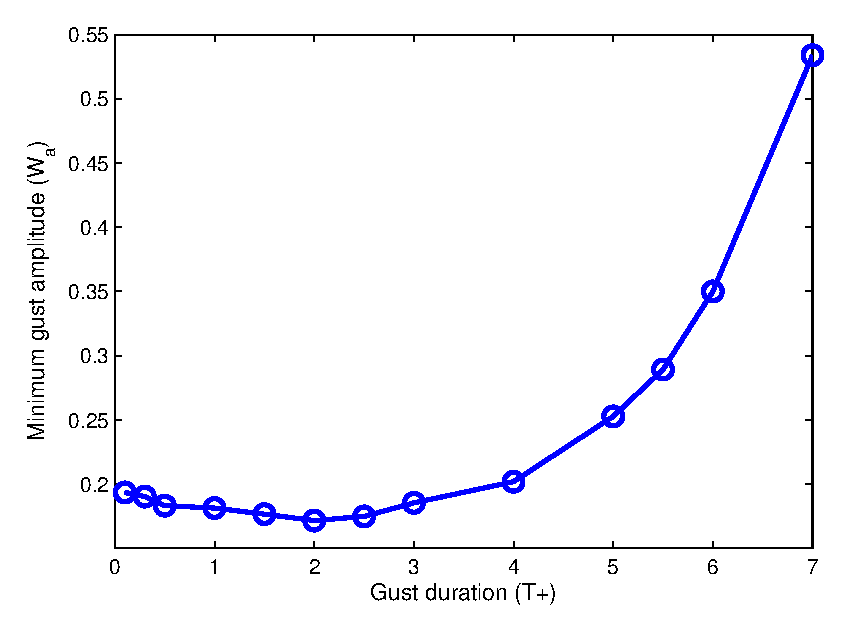
\includegraphics{./Figures/Vertical_gust_amplitude_vs_duration.eps}}
  \end{center}
  \caption{Influence of gust duration on the minimum gust amplitude for combined gusts}
  \label{fig:combined_amplitude_duration}
\end{figure}

\par Interestingly shorter gusts require less wind amplitude than the long ones.
This seems to indicate that most of the lost energy is due to the non-conservative drag force and not due to the downwind effects.
However the actual minimum gust amplitude required for neutral energy flight has a minimum for $2T$ long vertical gusts.

\par In figure \ref{fig:combined_amplitude_duration} This time no minimum is found.
This seems to reinforce the idea that the losses are mainly due to the energy dissipated by the drag since in this case the drag influence is mitigated by the horizontal component of the combined gust.

\par The diminishing gust amplitude required is an interesting phenomenon but can be fairly easily explained.
For a glider the only energy dissipation comes from the drag, in the cases we are considering the energy loss can be seen as a superposition of the losses due to simple cruse flight and the ones due to the maneuvering.
Since the total flight time during short gusts is shorter while the relative wind velocity remains more or less constant, the energy loss due purely to flying this long should be proportional to the flight time.
The energy input for this system is the wind gust itself is proportional to the force on the fluid times its velocity and the gust duration.
Since the force required to move the fluid is itself proportional to the derivative of the gust velocity the energy of the gust over a whole gust is in fact only proportional to the square of the gust amplitude.

\par This means that if the energy extraction efficiency was constant the value of $\frac{T_g0}{{W_g0}^2}$ should be constant for all the cases.


\begin{figure}[h!]
  \centering
  %\includegraphics{<+file+>}
  \caption{Energy extraction effectiveness}
  %\label{fig:<+label+>}
\end{figure}



\FloatBarrier


% get some commentary there

\Subsection{Influence of phase variation in the combined gust case}
For combined vertical and horizontal gusts another parameter can be changed.
So far the phase between the two components of the gust has been constant.

\par For this we define the phase $\phi$ as:

\begin{equation}
  \begin{array}[c]{c}
    W_g=W_a cos(2\pi T) \\
    U_g=W_a sin(2\pi T + \phi)
  \end{array}
  \label{eqn:combined_gust_phase}
\end{equation}

After Simulations are performed by 10 degrees steps with the following results.

\begin{figure}[ht]
  \begin{center}
    \scalebox{0.8}
    {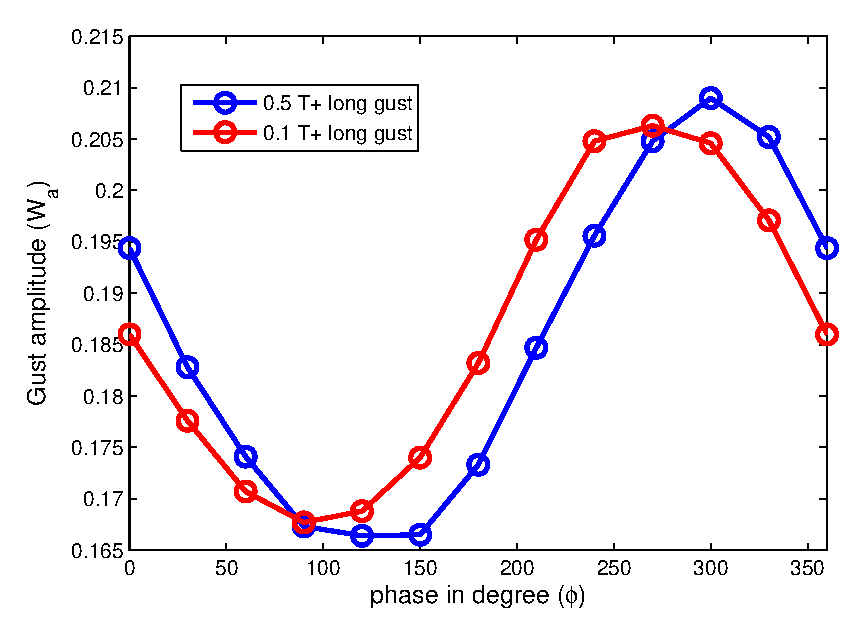
\includegraphics{./Figures/combined_gust_amplitude_vs_phase.eps}}
  \end{center}
  \caption{Influence of the phase between the component of the combined gust}
  \label{fig:combined_amplitude_phase}
\end{figure}

\par This clearly shows that our minimum gust amplitude for a 0 phase was actually close to the worst case possible.
The best case scenario is when the phase is around 90 to 120 degrees and the worst is around 270 to 300.

\FloatBarrier

\par We can see that the results are different for different gust durations.
One possible explanation for this is that at some point the inertia is too great and start to act as a low pass filter, introducing some phase shift in the trajectory. 



\Subsection{Maximum lift available effects}

\Subsection{Additional remarks}
As noticed by Lissaman the exact shape of the lift input isn't really important.
In his paper he approximated the input with a simple sinusoidal with amplitude and phase control, similar inputs in this simulation have produced minimum gust amplitude similar to the previous results.
This raises the hope that even very basic controllers should be able to improve UAV endurance.

% [DO I WANT TO  CHANGE THE PHASE TO ACTUALLY TEST IT !!!!]

\par While these results are supposed to be the optimal solution, it does not mean a controller can achieve such performances.
Even if the trajectory and lift curves are physically possible, the optimization algorithm assume a known gust shape and optimize all of the time points at once.
This means that contrary to a real controller the optimized trajectory can anticipate the wind change and preventively react.
Even if the wind gusts were perfectly sinusoidal, since a controller is casual it would not be able to anticipate.
Finally in a real life scenario the wind would of course not be a simple sinusoidal gust.

\par The simulation is also limited by its inability to account for the moment of inertia along the pitch axis.
Even is part of the lift change can be handled by the active flow control system, at low angle of attack, most of the lift comes from the changes in $\alpha$.

\par Even with all this limitations these results provide good insight into what would be needed implement energy extraction trajectories in UAVs.




\Chapter{Modelling of the Lift coefficient under unsteady pitching motion} \label{Ch:gkmodel}

\Section{The Goman and Khrabrov model}

\Subsection{Motivation}
In their 1994 paper entitled ``State-Space Representation of Aerodynamic Characteristics of an Aircraft at High Angle of Attack'' \cite{GK} Goman and Khrabrov introduce a new model for characterizing the lift and moment coefficients for slender delta wings.
Their goal was to study the stability of delta wing fighter jets where maneuverability is important, and to link it to physical fluid dynamic phenomenons such as vortex breakdown or flow separation.

\par The classical stability analysis method relies on a Taylor series expansion of the aerodynamic coefficients.
% maybe put an example here.
This linear representation is relatively accurate for fully attached flow but the model breaks down at higher angle of attack when separation occurs.
In the semi separated region the aerodynamic effects are mainly driven by the degree of flow separation happening on the wing.
For this reason they chose to define $C_l$ as a function of $\alpha$, the angle of attack, and a state variable $x$ representing the degree of separation.
This degree of separation can be defined as the position of the vortex breakdown point if you are looking at delta wings, or the position of the reattachment point in the case of 2D airfoils.
This allows for a model tightly defined by the physics of the flow.


\Subsection{Flow physics and state variables}
Since this study was performed with a 2D NACA0009 airfoil, we define the state variable $x$ as the position of the reattachment point.
Its value linearly change from 1 when it is situated at the leading edge to 0 when it gets to the trailing edge and beyond.
For quasi-steady cases separation point is a function of the angle of attack. If we define $x_0$ as the separation point position in a quasi-steady situation then

\begin{equation}
  C_l^{qs} = f(\alpha,x_0(\alpha))
  \label{eqn:qs_Cl}
\end{equation}

The unsteady part of the flow physics can be divided into two groups of phenomenons.

\par The firsts are the effects of the angle of attack variation speed on the position of the separation point.
Goman and Khrabrov argue that this is roughly proportional to the pitch rate $\dot{\alpha}$ and as such they can be included by modifying the quasi-steady state value by using $x_0 (\alpha - \tau_2 \dot{\alpha})$ 

\par The second phenomenon is due to the dynamics of the separated flow.
The flow has a certain relaxation characteristic under a disturbance input.
This can be modeled using a first order differential equation.

\begin{eqnarray}
  \tau_1 \frac{dx}{dt} +x = x_0(\alpha - \tau_2 \dot{\alpha}) 
  \label{eqn:state_variable}
\end{eqnarray}

\Section{Experimental Setup}

\Subsection{Equipment and facilities}

\begin{figure}[h]
  \begin{center}
%\includegraphics{<+file+>}
  \end{center}
  \caption{Airfoil model inside the wind tunnel}
  \label{fig:wind_tunnel}
\end{figure}

All of the experimental part of this research was performed into the Andrew Fejer Unsteady Wind Tunnel at the Illinois Institute of Technology, Chicago.
This is a low velocity wind tunnel with a 60cm by 60cm test section.
The wind tunnel is mainly used for unsteady aerodynamic studies.
Airfoils are mounted on a motorized sting outfitted with two linear electric servo-motors.
These servos are powered by an amplifier with a integrated PID system and driven by an analog voltage input signal proportional to the desired position.

\begin{figure}[h]
  \begin{center}
%		\includegraphics{<+file+>}
  \end{center}
  \caption{Pitching and plunging mechanism}
  \label{fig:pitching_mechanism}
\end{figure}

As seen on figure \ref{fig:pitching_mechanism} combining the motion of the front and back servo allows for the wing to be plunged as well as pitched around a range of axis.
The tunnel is also equipped with a system of shutters that can be used to create wind gusts.
However this feature will not be used in this project.

\par The input signal for the servos is made with Simulink\textsuperscript{\textregistered} and fed through D-Space\textsuperscript{\textregistered} as an analog voltage.

\par Several sensors are used for data acquisition.
A pair of linear potentiometers measures the position of the servos in order to get the airfoil pitch angle.
The flow speed is measure via a Pitot tube and pressure transducer plugged into a acquisition box.
In parallel to this acquisition box the forces exerted on the airfoil can be measured.
A piezoelectric ATI Nano17 force balance seats between the sting and the airfoil.
This sensor measures both absolute forces and moments along 3 different axis.

\par The wing is made out of balsa wood with a 3D printed leading edge housing the active flow control system.
This system will be described in more detail in the appropriate chapter.
The structure is wrapped in mono-coat, a heat-shrunk plastic film.
Its chord length is 245mm its width 560mm with a NACA0009 profile.
It connects to the force balance at a point at 25 percent of the chord.
The maximum was made to keep the weight and moment of inertia as small as possible to minimize the inertial effects when the wing is moving.


\FloatBarrier

\Subsection{Experimental procedure and data processing}
Different pitch input have been tried.
There was some fears at first that if the pitching axis wasn't on the axis symmetry, at the quarter chord of the airfoil, additional aerodynamic phenomenon would affect the data.
After testing different pitching input that placed the rotation axis either at the top of the front servo, at the top of the force balance or at the top of the back servo,  it was determined that the optimal way to drive the pitching mechanism was to move only the back servo.
Other input method induced to much mechanical vibrations and did not seems to make any difference aerodynamically.

\par The amplifier driving the electric servos has its own PID control system, however even after careful tunning some error exists between the commanded angle of attack and the actual angle of attack.
To negate that effect the actual servo position, as given by the potentiometers, is used for our measurements.
This data is used to transform the normal and tangent force into lift and drag (via a simple rotation matrix). 
They are then normalized to get the aerodynamics coefficients.

\par Unless specified otherwise, all the acquisitions have been done at a flow speed of 3m/s which correspond to a Reynolds number of 50000.

\par For each experimental case the force balance as well as the servo position and a synchronization signal are simultaneously acquired.
A first offset with the tunnel off and the wing pitching is taken to let us get the force balance offset as well as record the inertial effects.
Even tho the wing is only weighing around 300 grammes, these inertial effects represent the majority of the forces measured by the force balance.
Moreover some of the force measured come from the springiness of the cables used for the active flow control part.
After the first offset the real case is taken, followed by a second offset to account for the drift in the force balance measurement sometime seen over the course of several minutes.

\par During each acquisitions at least 50 cycles are recorded.
This allows us to perform what we call phase averaging.
This is done by slicing the files into individual cycles (thank to the synchronization signal) and then making an average of these cycles.
With this technique the signal to noise ratio of greatly improved.
Once this has been done with the 2 offsets and the proper acquisition itself, aerodynamic forces are obtained by subtracting the offsets.
All this processing is done with Matlab\textsuperscript{\textregistered}. 

\par The servo actuation system has a small but noticeable dead band as well as a delay between the input and output.
This makes the actual pitching motion slightly different from the input.
To account for that the actual measured pitch angle is used as an input of the GK model when we want to compare its prediction with the experimental data.

\par Finally the GK model itself is also implemented in Matlab.
The code can be seen in annex \ref{ch:GK_code}.



\FloatBarrier


\Section{Adapting the GK model to the NACA0009}

\Subsection{Steady lift and stalling behavior}
With the basics of the GK model defined, the goal is now to adapt it to our objectives.
If this model is to be used for optimization purposes the drag also needs to be calculated.
The original model defined by Goman and Khrabrov was included the lift and pitching moment coefficients.
Similarly to their model the assumption is made that the lift and drag coefficients share the same state variable.
As such we define $f$ and $g$ as

\begin{equation}
  \begin{array}[c]{c}
    C_l=f(\alpha,x) \\
    C_d=g(\alpha,x)
  \end{array}
  \label{eqn:lift_drag_functions}
\end{equation}

\par The other difference with their case study is that we are considering a 2D airfoil whereas they modeled a 3D delta wing.
This means that we can't reuse the same lift function $f$ as the original paper.

\par In order to get an accurate equation for the lift and drag a quasi-steady map of the lift and drag coefficients is made.
This map is done by very slowly (0.1 degree per seconds) pitching the wing between -5 and 25 degrees.
The free stream speed has to be corrected to account for the flow slowing down during the higher blockage ratio at high angle of attack.

\begin{figure}[ht]
  \begin{center}
    \scalebox{0.8}
    {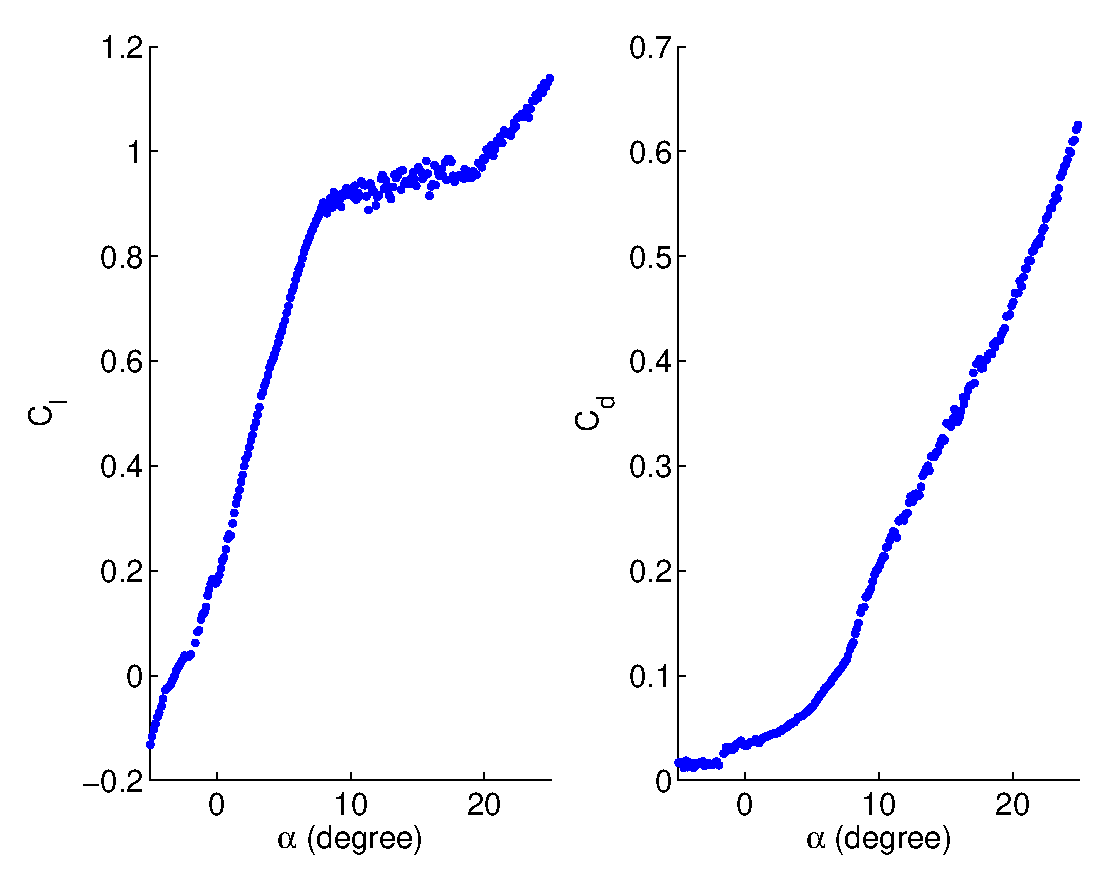
\includegraphics{./Figures/NACA0009_steady_map_Cl_Cd.eps}}
  \end{center}
  \caption{Lift and drag coefficient in the quasi-steady case}
  \label{fig:QS_Cl_Cd_vs_alpha}
\end{figure}

\par Figure \ref{fig:QS_Cl_Cd_vs_alpha} shows how the aerodynamics behave for our NACA0009 airfoil.
The lift coefficient is close to a clean linear function when the flow is attached.
The separation happens around 8 degrees and the lift coefficient remains constant in the 10 to 20 degrees zone when the flow is partially separated.
At higher angle of attack the flow is totally separated and $C_l$ is once again proportional to $\alpha$ but with a different slope this time.
Even though the NACA0009 has a symmetric profile the measured lift coefficient for a angle of attack of zero is not null.
It is suspected that the sting onto which the airfoil is fixed may disturb the flow and cause this asymmetry.
Moreover this curve differs slightly from the ones found in the literature.
Once again this can be attributed to the experimental setup; other than the sting effects the couple of millimeters of clearance between the wall of the wind tunnel and the edge of the airfoil are probably to blame as they induce some 3D effects.
These gaps are necessary for to allow for the both pitching and plunging of the wing.

\par From this static map we can approximate the part where the flow is still attached (<8 degrees) by 

\begin{equation}
  \begin{array}[c]{c}
    C_l= 2 \pi \cdot \alpha + C_l0 \\
    C_d= \frac{C_l^2}{2G_{max}} + C_d0
  \end{array}
  \label{eqn:attached_Cl_and_Cd_vs_alpha}
\end{equation}

Which is remarkably close to the classical theoretical result for a 2D airfoils in a ideal inviscid attached flow.

\Subsection{State variable approximation}
When the flow is still attached the value of $x$ is 1. 
This means that we are considering the separation point to be at the trailing edge.
Similarly when the flow is totally separated the separation point is at the leading edge and $x=0$.
Since for totally separated flow the slop of the lift coefficient as a function of $\alpha$ can be approximated to about $0.4$ of the slope for the attached flow, we choose to use the following equation for the lift over the whole range of angle of attack. 

\begin{equation}
  C_l(\alpha,x)=2 \pi \cdot \alpha (0.6 x + 0.4) + C_l0
  \label{eqn:Cl_function}
\end{equation}

\par By inverting this equation the value of $x_0$ can then be adjusted so that the output of this function matches the experimental data. 
The resulting profile for $x_0(\alpha)$ can be seen in figure \ref{fig:x_0_vs_alpha}

\begin{figure}[h]
  \begin{center}
    \scalebox{0.8}
    {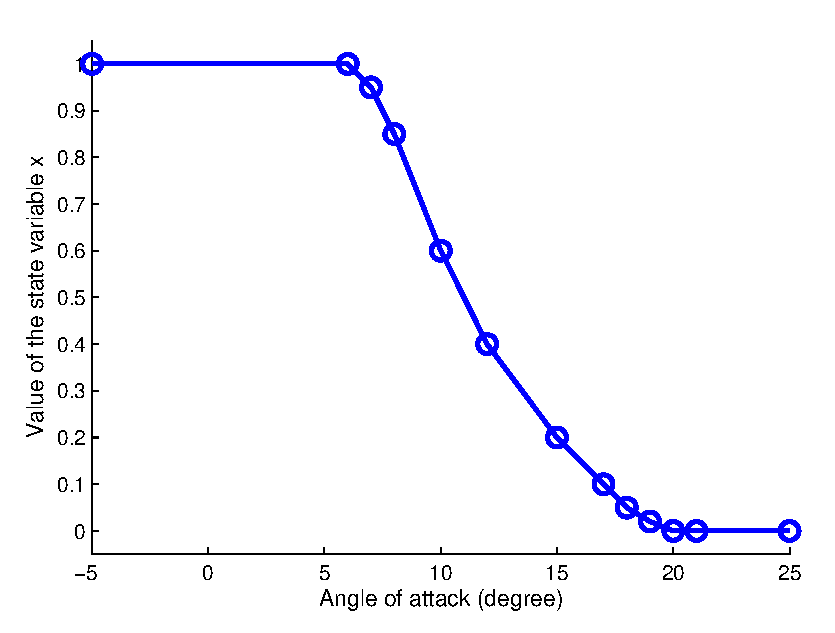
\includegraphics{./Figures/x_0_vs_alpha.eps}}
  \end{center}
  \caption{Quasi-steady profile for the state variable $x$}
  \label{fig:x_0_vs_alpha}
\end{figure}

\FloatBarrier
With this profile we get a good approximation of the experimental $C_l(\alpha)$ (cf figure \ref{fig:GK_Cl_vs_alpha}) for quasi steady cases.

\begin{figure}[h]
  \begin{center}
    \scalebox{0.6}{
      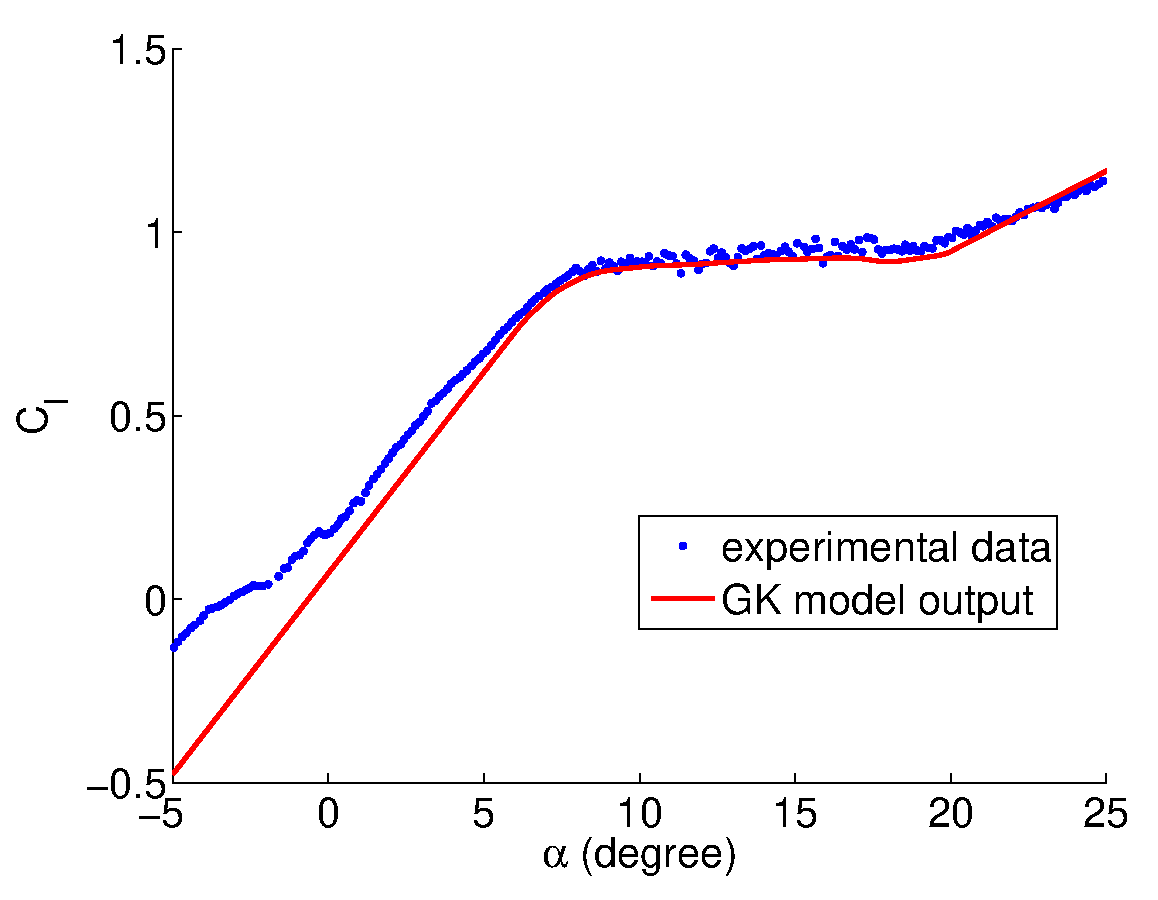
\includegraphics{./Figures/GK_cl_vs_alpha.eps}}
  \end{center}
  \caption{Comparison between the experimental and model quasi-steady lift}
  \label{fig:GK_Cl_vs_alpha}
\end{figure}

\par The assumption that the drag share the same state variable as the lift is confirmed when the following equation produces similarly accurate results compared to experimental data, as seen on figure \ref{fig:GK_Cd_vs_alpha}.

\begin{equation}
  C_d(\alpha,x)= \frac{ \left( \left( 2 - x \right)C_l \right)^2 }{2 G_{max}} + C_d0
  \label{eqn:Cd_function}
\end{equation}

\begin{figure}[h]
  \begin{center}
    \scalebox{0.6}
    {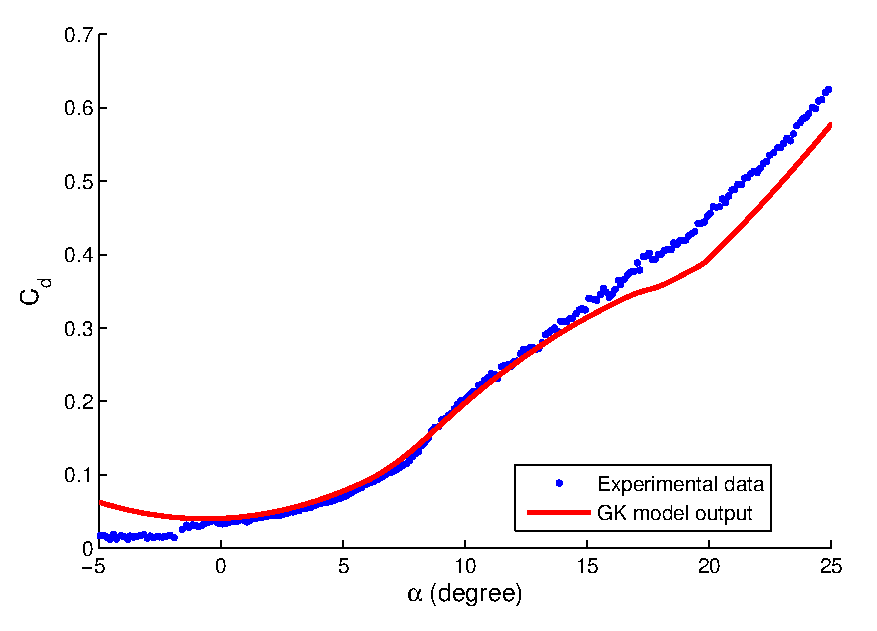
\includegraphics{./Figures/GK_cd_vs_alpha.eps}}
  \end{center}
  \caption{Comparison between the experimental and model quasi-steady drag}
  \label{fig:GK_Cd_vs_alpha}
\end{figure}

\par These two relatively simple equations shows that a physics based GK model can be implemented for both lift and drag and that they indeed depend on the same state variable.
The two time constants $\tau_1$ and $\tau_2$ will be determined in the next section when the wing undergo unsteady pithing.

\FloatBarrier
\Section{Model validation}

\Subsection{Time constants}
While the ability to predict lift and drag based on separation can be useful, the real strength of the GK model resides in its ability to work on unsteady cases.
The first step is to determine the 2 $\tau$ time constants. 
To do that a series of pitching cases are performed. 
The pitching inputs are the following

\begin{equation}
	\alpha\left( t \right)= A \sin \left( 2 \pi \frac{t}{f} \right) + \alpha_0
	\label{eqn:pitch_input}
\end{equation}

With $A=2^\circ$ and $\alpha_0=12^\circ$.
The frequency $f$ is set to 0.25, 0.5, 1 and 2 Hz (respectively K of 0.064, 0.128, 0.257 and 0.513)

\begin{figure}[h]
  \begin{center}
    \scalebox{0.8}  
    {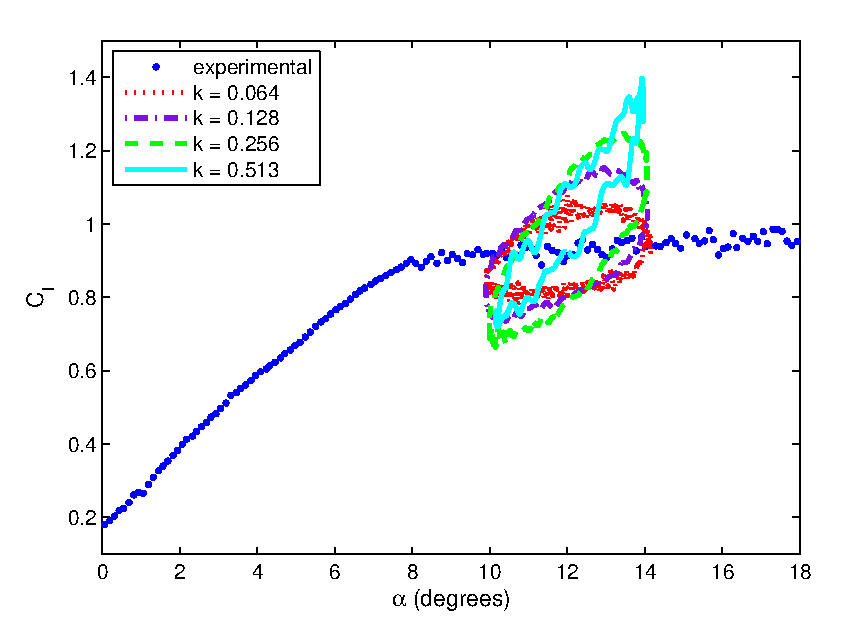
\includegraphics{./Figures/Pitching_allcases_CL_12_amp_2.eps}}
  \end{center}
  \caption{Unsteady effects on the lift of sinusoidal pitching around 12 degree} 
  \label{fig:Pitching_allcases_Cl_12}
\end{figure}

\begin{figure}[h]
  \begin{center}
    \scalebox{0.8}  
    {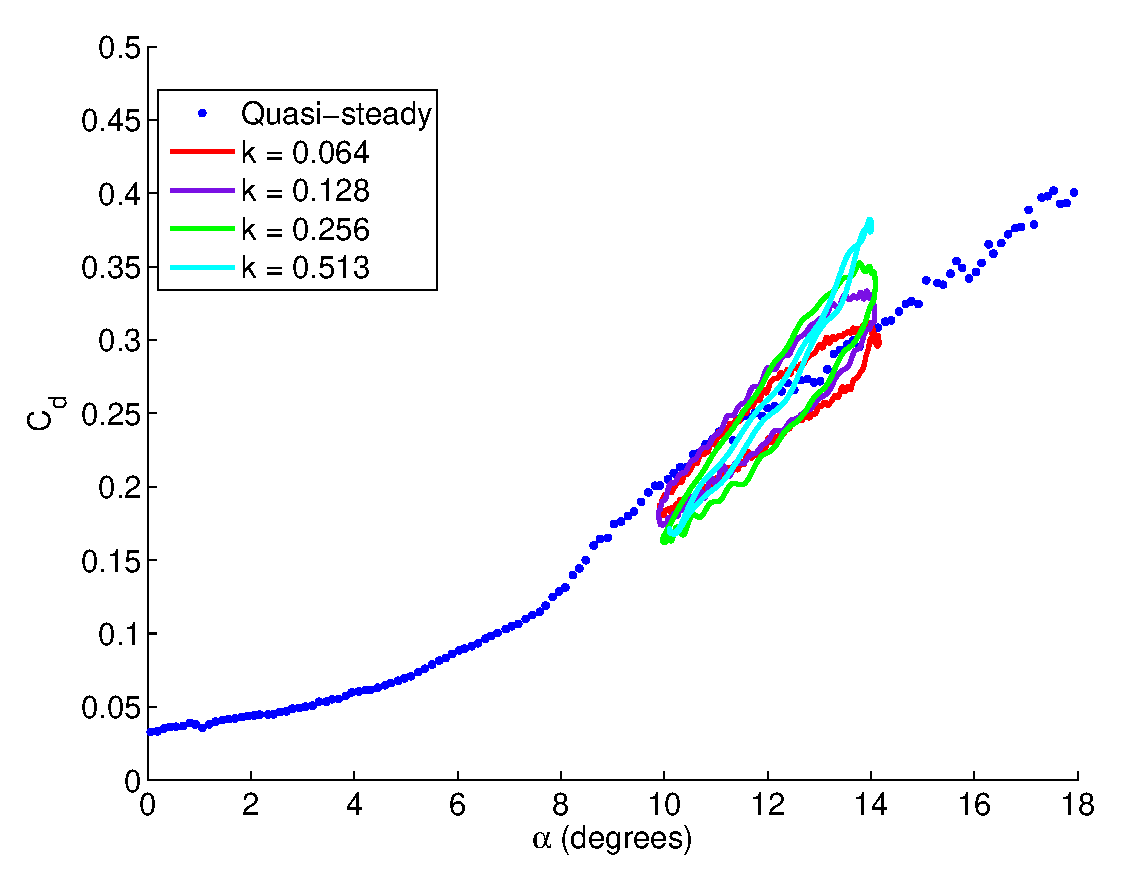
\includegraphics{./Figures/Pitching_allcases_CD_12_amp_2.eps}}
  \end{center}
  \caption{Unsteady effects on the drag of sinusoidal pitching around 12 degree} 
  \label{fig:Pitching_allcases_Cd_12}
\end{figure}

\FloatBarrier

\par On these figures it is easy to notice the influence of the time delays on the aerodynamic coefficients.
At the lower frequencies the loops are quite open and a significant difference exists between the lift obtained during the pitch up and the pitch down phase.
These lift value circulate on these loops rotating in an anti-clockwise direction.
This means that the lift is higher during pitch down maneuver.
Contrastingly this behavior disappears at higher frequencies.
For K values of 0.257 and 0.513 the difference between the pitch up and pitch down is lower.
However the lift variation amplitude is more pronounced in those cases.

\par Before using the Gk model as a predictive tool the time constants need to be found.
This is done by trial and error.
The two time constants are determined manually and are tuned to produce the best results at the different frequencies tested.
$\tau_1$ is found to be equal to 3.06 t+ (0.25s) and $\tau_2$ is 4.29 t+ (0.35s).


\par The reason for the difference in behavior between the high and low frequencies is that at low frequencies the flow has the time to separate from the airfoil, this can be checked by the fact that state variable $x$ is driven by the time constant $\tau_1$.
The characteristic frequency corresponding to this time constant is about $k=1.02$.
For $k$ values of 0.257 and up, the low order filter described by the state variable equation \ref{eqn:state_variable} start to be more apparent.
A higher frequencies the flow doesn't have the time to separate and the lift coefficient is mainly driven by the $2\pi\alpha$ multiplier.
This can be seen on the by overlaying a line with a $2\pi\alpha$ slope on the results.

\par Theoretically the value of $\tau_1$ could be found by analyzing the output of small step input for the angle of attack.
In this situation $\dot{\alpha}$ at the time the step is taken but it doesn't last long enough affect the value of the state variable since the first order differential equation for $x$ acts as a low pass filter.
This means that for a small step $C_l$ from 12 to 13 degrees the output lift looks like the following figure.

\begin{figure}[h]
  \centering
  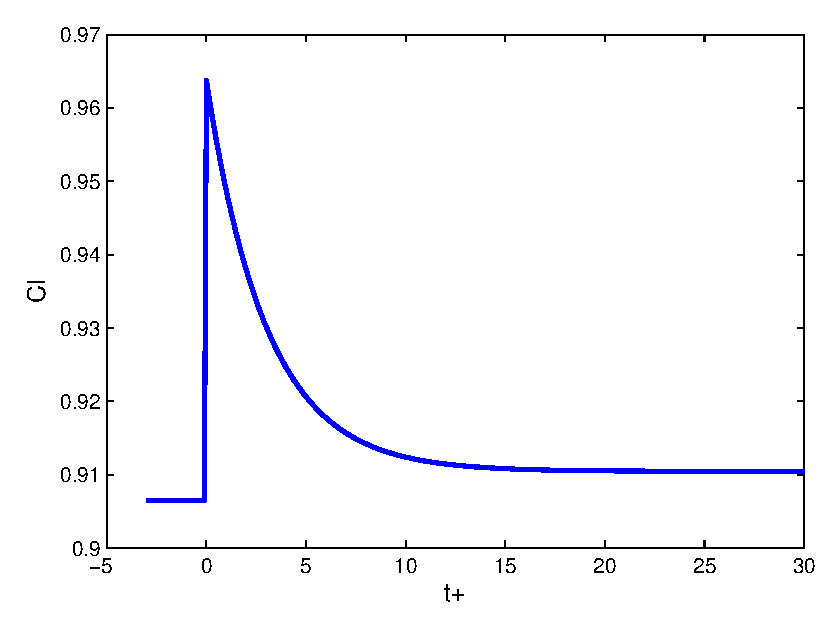
\includegraphics{./Figures/Cl_vs_tplus_step_12to13.eps}
  \caption{Cl behavior for a instantaneous step from 12 to 13 degrees at $t+=0$, as simulated by the GK model}
  \label{fig:Cl_for_alpha_step}
\end{figure}

\par From this classical methods used to find the time constant for first order system can be used.
As you can see in the figure \ref{fig:tau_1_identification}, the $\tau_1$ constant found from the GK model output is really close to the one used in the model.

\begin{figure}[h]
  \centering
%  \includegraphics{<+file+>}
  \caption{Identification of $\tau_1$ from the step response}
  \label{fig:tau_1_identification}
\end{figure}	

\par While this method is fine in theory, it is impossible to implement experimentally.
The force balance used to measure lift and drag is very fragile so a fast step could be enough to break it.
Furthermore any slower of even smoothed step input modifies the lift response enough to make the time constant identification impossible.
While this method is unpractical for experimental cases it should be applicable in the case of CFD simulations.

\Subsection{Model comparison at different frequencies mean angle and amplitudes}
Now that the model is complete its accuracy can be checked.
The most obvious result is that the shape of the lift and drag versus angle of attack curves are similar to the experimental results.

\begin{figure}[h]
  \begin{center}
    \scalebox{0.6}{
      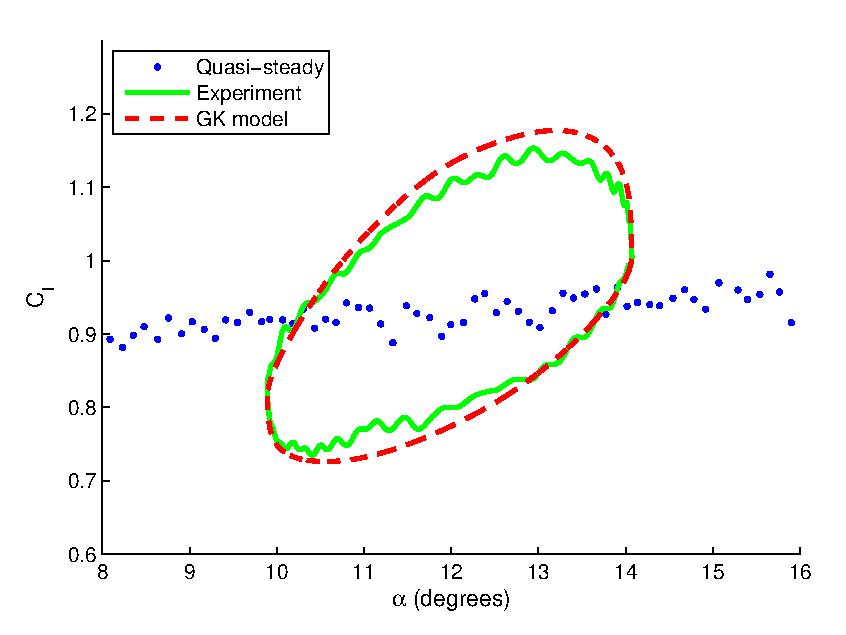
\includegraphics{./Figures/Cl_u=3_meanaoa=12_amp=2_freq=0p5.eps}}
  \end{center}
  \caption{Comparison of experimental lift coefficient and model prediction after tunning of the time constant at k =0.128}
  \label{fig:Cl_u=3_meanaoa=12_amp=2_freq=0p5}
\end{figure}

\begin{figure}[h]
  \begin{center}
    \scalebox{0.6}{
      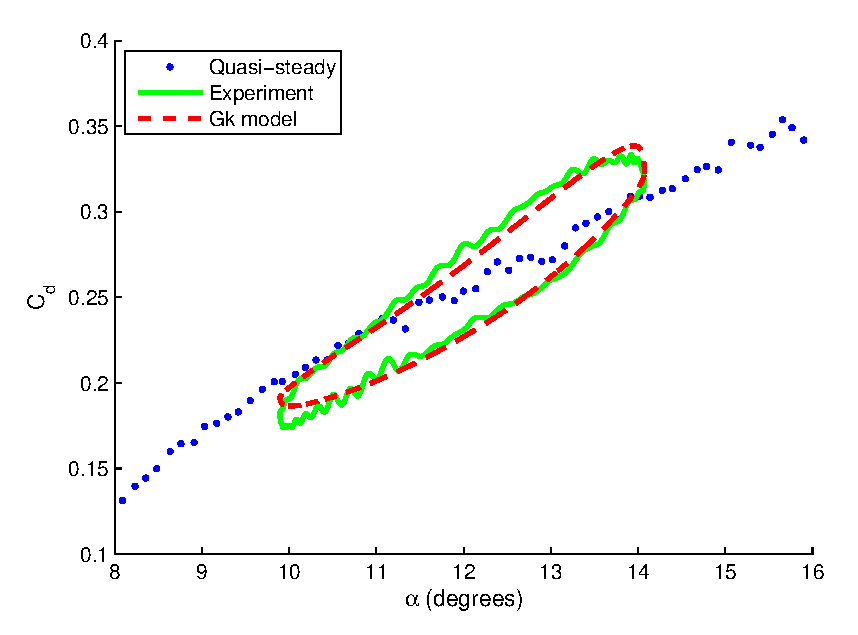
\includegraphics{./Figures/Cd_u=3_meanaoa=12_amp=2_freq=0p5.eps}}
  \end{center}
  \caption{Comparison of experimental drag coefficient and model prediction after tunning of the time constant at k =0.128}
  \label{fig:Cd_u=3_meanaoa=12_amp=2_freq=0p5}
\end{figure}

\FloatBarrier

\par This behavior can be checked for other frequencies as well.

\begin{figure}[h]
  \begin{center}
    \scalebox{0.6}  
    {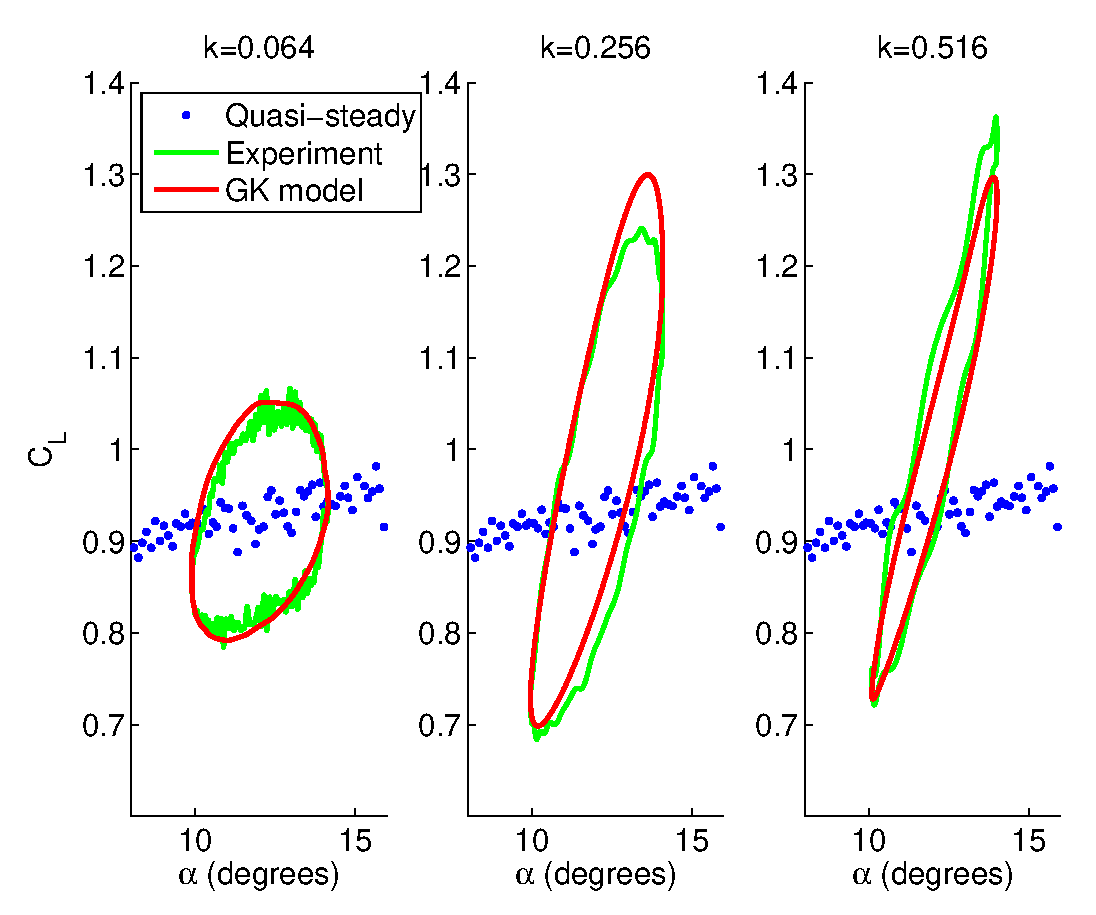
\includegraphics{./Figures/Pitching_allcases_GK_CL_12_amp_2.eps}}
  \end{center}
  \caption{Lift measurement and prediction during sinusoidal pitching around 12 degree} 
  \label{fig:Pitching_allcases_GK_Cl_12}
\end{figure}

\begin{figure}[h]
  \begin{center}
    \scalebox{0.6}  
    {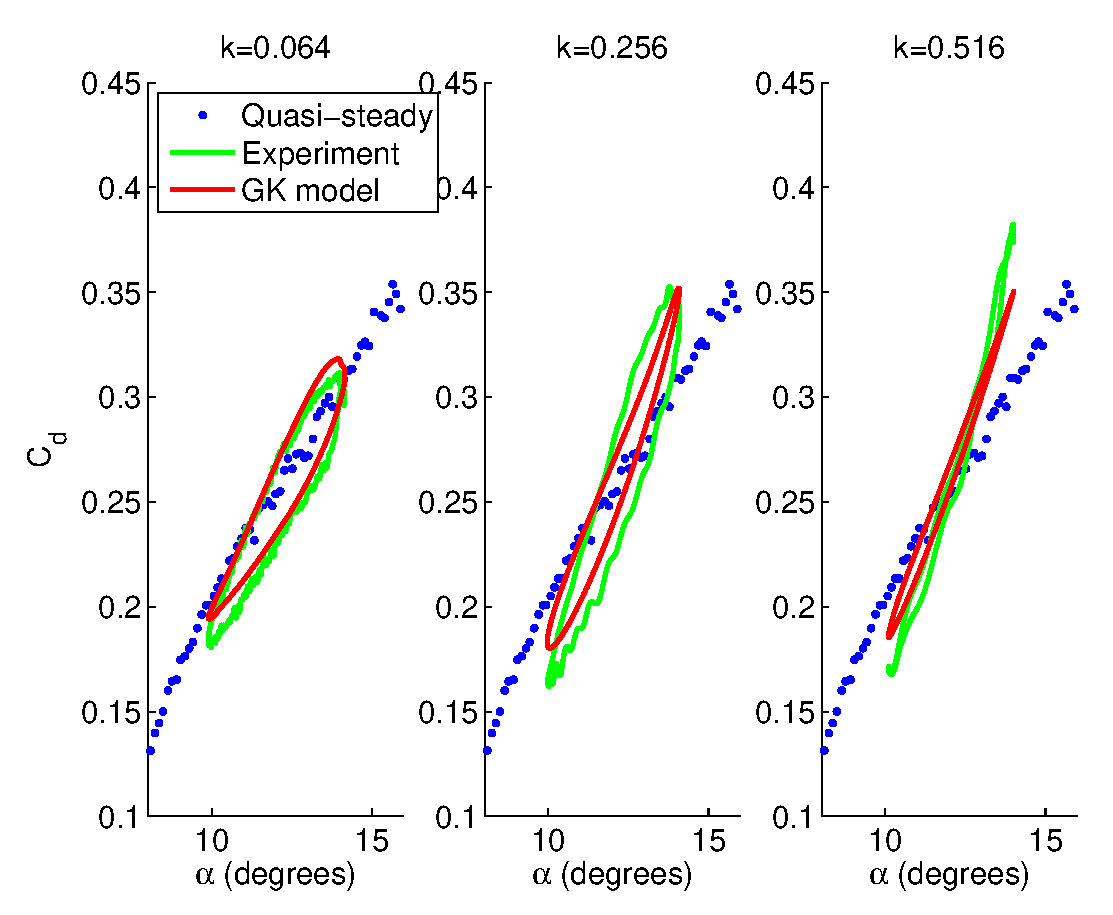
\includegraphics{./Figures/Pitching_allcases_GK_CD_12_amp_2.eps}}
  \end{center}
  \caption{Drag measurement and prediction during sinusoidal pitching around 12 degree} 
  \label{fig:Pitching_allcases_GK_Cd_12}
\end{figure}

\par Similarly another set of acquisitions is made at a mean angle of 10 degrees (see figures \ref{fig:Pitching_allcases_GK_Cl_10} and \ref{fig:Pitching_allcases_GK_Cd_10}).
For some unknown reason the model does not seems to model the behavior in the drag very well at this frequency.

\begin{figure}[h]
  \begin{center}
    \scalebox{0.6}  
    {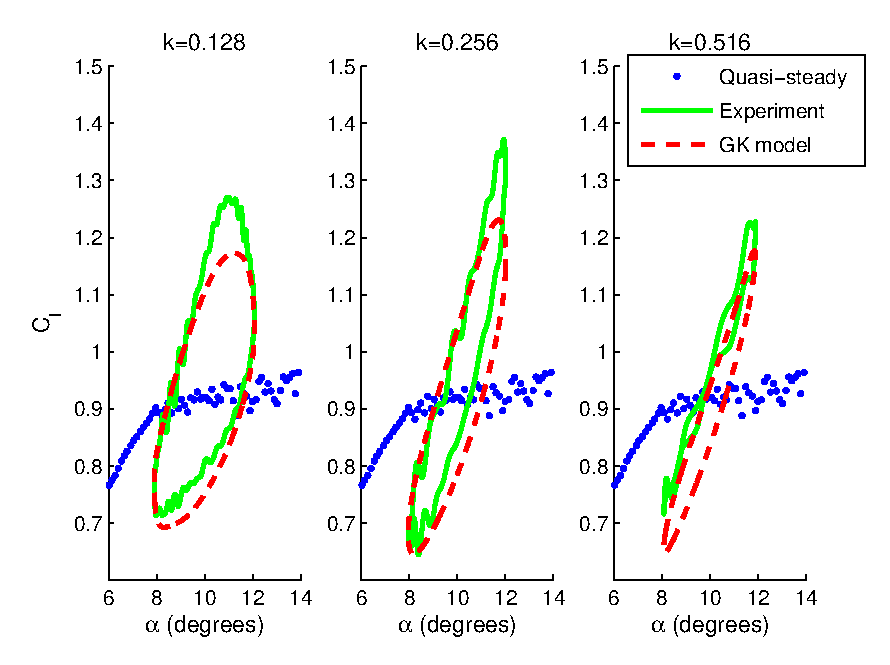
\includegraphics{./Figures/Pitching_allcases_GK_CL_10_amp_2.eps}}
  \end{center}
  \caption{Lift measurement and prediction during sinusoidal pitching around 10 degree} 
  \label{fig:Pitching_allcases_GK_Cl_10}
\end{figure}

\begin{figure}[h]
  \begin{center}
    \scalebox{0.6}  
    {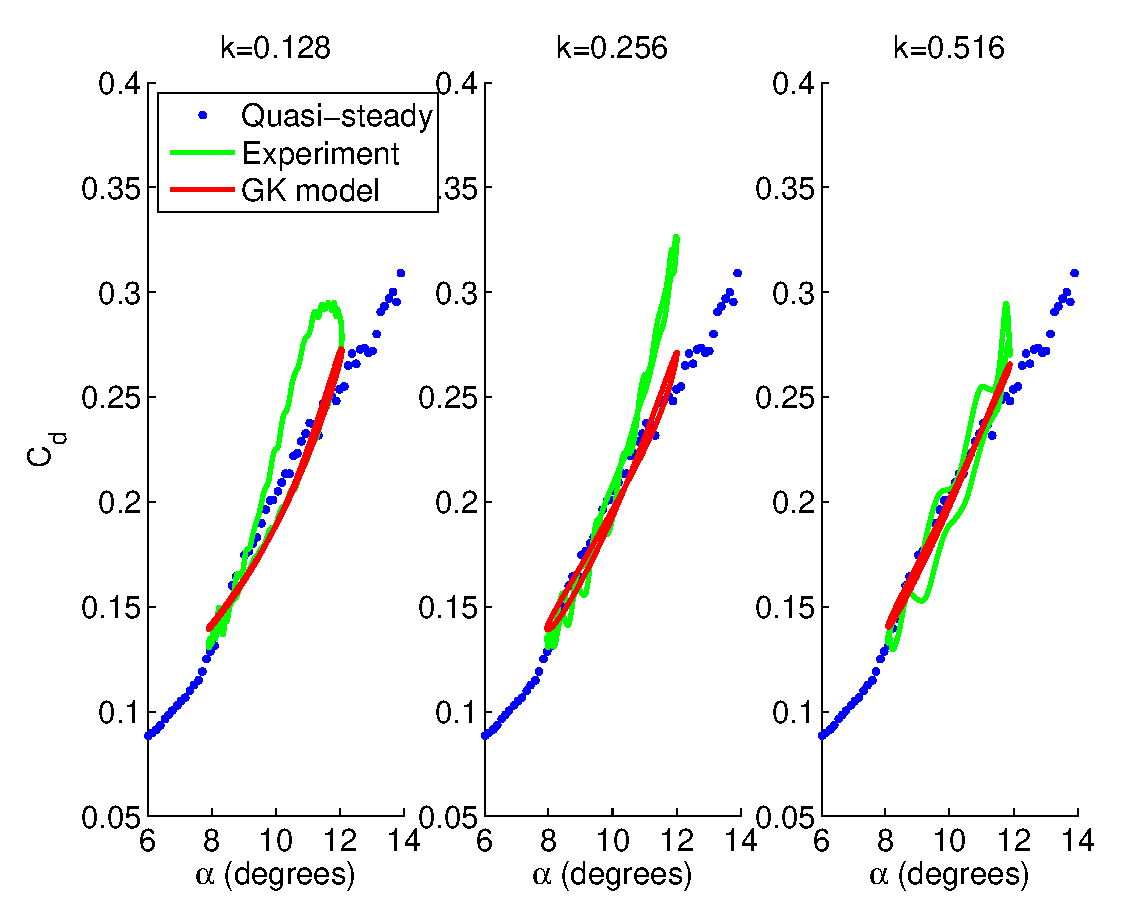
\includegraphics{./Figures/Pitching_allcases_GK_CD_10_amp_2.eps}}
  \end{center}
  \caption{Drag measurement and prediction during sinusoidal pitching around 10 degree} 
  \label{fig:Pitching_allcases_GK_Cd_10}
\end{figure}

\FloatBarrier

\par The area around 8 degrees is interesting because this is where the flow just starts to be get separated.
The transition between attached flow and separated flow means that the state variable $x$ shouldn't have any effect for the lower angles and as a consequence the loop seen in the $C_l$ versus $\alpha$ plots should be ``pinched'' on its left side.
This can be further illustrated by plotting the value of the state variable during this kind of maneuvers, it is constrained by the saturation of this value at one.
This kind of behavior is particularly apparent on high amplitude (tens of degrees) pitch maneuver as it is seen in the original Goman and Khrabrov paper.
The behavior is comparable at K of 0.257 and 0.513 but the drag has a noticeably different shape at K of 0.128.

\par Another obvious parameter to check for our model is the amplitude of the oscillations.
The amplitude is set to a range from 1 to 4 degrees at different mean angle of attack.
The predictions still reasonably match the experimental results. 

% divers figures

\Subsection{Non-periodic pitch input}
To simulate a more realistic pitch profile, a pseudo-random pitch profile is designed.
The input is constructed as seen in equation \ref{eqn:random_pitch_input} with a randomized phase difference $\varphi_i$ between each harmonic components.

\begin{equation}
	\alpha_{random}= \frac{\sum_{i=1}^{10} \sin (\frac{2 \pi t}{f_i} + \varphi_i)}{B} + \alpha_{0}
	\label{eqn:random_pitch_input}
\end{equation}

The frequency are regularly spaced between 0.25 and 2Hz and the constant $B$ is chosen to make sure the maximum deviation from the $\alpha_0$ value is no more than 2 degrees.
This is done so that the bandwidth of the input signal is limited to reasonable levels and to keep the force balance safe.

\begin{figure}[h]
  \begin{center}
    \scalebox{0.6}  
  {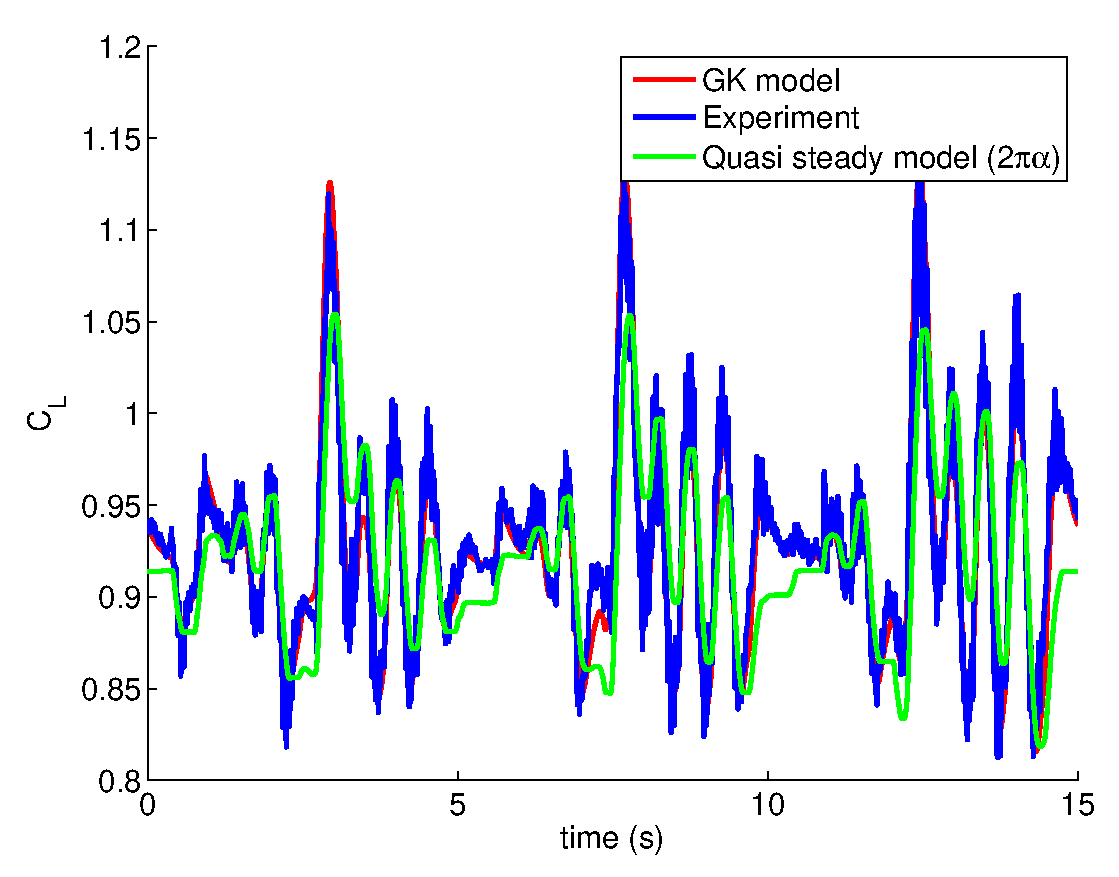
\includegraphics{./Figures/Cl_u=3_meanaoa=12(15seconds)_amp=2_freq=2p0.eps}}
  \end{center}
  \caption{Unsteady effects of random pitching on the lift}
  \label{fig:Pitching_random_Cl_12}
\end{figure}

\begin{figure}[h]
  \begin{center}
    \scalebox{0.6}  
  {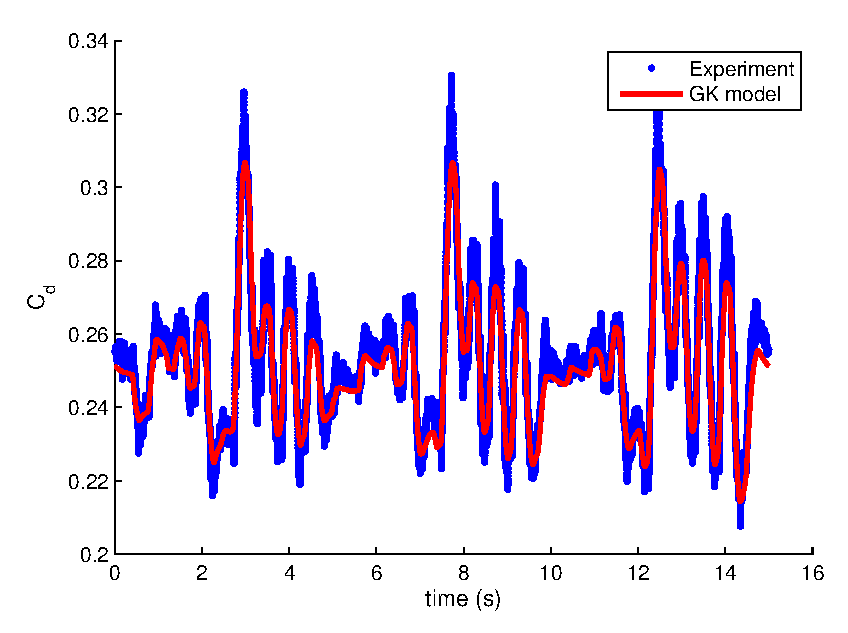
\includegraphics{./Figures/Cd_u=3_meanaoa=12(15seconds)_amp=2_freq=2p0.eps}}
  \end{center}
  \caption{Unsteady effects of random pitching on the drag}
  \label{fig:Pitching_random_Cd_12}
\end{figure}

\par The accuracy of these results means that this model could be used in real time during arbitrary pitching maneuvers.
This is potentially very useful since a lot of systems rely on the periodicity of the pitching motion to predict the lift and can be inaccurate in case of non periodic disturbances such as wind gusts changing the effective angle of attack.

\FloatBarrier

\par This model is producing accurate results that account for both the dynamic effects and the flow separation.
Moreover the procedure is light enough to be implemented into the optimization algorithm without increasing too much the computation cost


\Section{Model limitations}

While this model produces impressive results for a lot of different cases it is not without its limitations.

\Subsection{Inertial and added mass effects} \label{subs:added_mass}

One of the biggest issue of the experimental part for the pitching experiment are the inertial effects due to the mass of the wing being thrown around.
These inertial effects represent very high loads compared to the actual aerodynamic loads.
To these we get the weight of the wing being added to the force balance measurement.

\par Since we are only interested in the aerodynamic forces we need to eliminate these mechanical forces.
As explained before we remove these by averaging over several cycles both an acquisition with the tunnel on and one without the model on.
Assuming that the inertial effects are reproducible (this has been a fairly solid assumption) then the forces due to the momentum and weight are removed.
However the acquisition done when the wind tunnel is not running are not done in vacuum.
As such the added mass effects are subtracted from the final data.

\Subsection{Center of rotation}

Traditionally whenever span-wise data are considered, all all moments and rotation centers are taken at the quarter chord point.
With our double servomotor system we are able to find a relation which will allow us to rotate the wing around any arbitrary point (provided it is within the mechanical range of the actuators).
A batch of acquisition was performed with the rotation point set at the emplacement of the force balance to minimize the effects of inertial tangential and normal forces on the measurements.
However the results were deemed not as good as simply moving the back servo.
The simultaneous motion of the two servos introduce a lot of vibrations, especially when small and slow motions are needed.
This is due to the electric servos being based on stepper motors and the fact that the two servo rods are very close together.

\par Attempts to move only the back servo (instead of the front) produced worst data than moving the back one.
A possible explanation is that the front servo has to support the whole wing and sting assembly whereas the back one has a much lighter load.
Under this higher load the servo positioning system is not as precise.

\par Any unwanted forces created by rotating the airfoil in front of the quarter chord point should get subtracted by the procedure described in the previous section \ref{subs:added_mass}.

%servo drive and stuff
\Chapter{Trajectory optimization with the unsteady model}
\Section{Implementation in the energy extraction algorithm}

\par As seen in the previous chapter the optimization process for the energy extraction trajectory only requires a way to calculate the relationship between the lift and drag coefficient.
Since in our case these 2 variables depend only on the angle of attack and its change rate over time, it is fairly easy to implement it into the algorithm.
However the non dimensional time constant are different, the energy extraction one consider the optimal glide speed and the gravity acceleration whereas the one used for the GK model uses the flight speed and the chord length.

\Subsection{Relation between the different time scales}
As said before the time scale used in the two models are different.
To solve this issue the ratio of the two time constants are plotted (see figure \ref{fig:T_t+_ratio}) for a wide variety of flying objects.

\begin{equation}
  \frac{T}{t+}=\frac{V_{opt}}{g} \cdot \frac{U}{c}
  \label{eqn:T_t+}
\end{equation}

Or if the aircraft flies near its optimal glide speed

\begin{equation}
  \frac{T}{t+}=\frac{V_{opt}^2}{g \cdot c}
  \label{eqn:T_t+_ratio}
\end{equation}

This ratio happens to be the Froude number.


\begin{figure}[ht]
  \begin{center}
    %\includegraphics{<+file+>}
  \end{center}
  \caption{T to t+ ratio for divers flying objects}
  \label{fig:T_t+_ratio}
\end{figure}

\par It is interesting to notice that this ratio is in the same order of magnitude for all these objects.
The value of 90 is chosen as a default for this ratio as it represent a good average of the data compiled.


\par Another issue is that the GK model is dependent on the initial value of the state variable $x$.
The initial value of $x$ is taken as the quasi-steady value.
To minimize the effect of the transition from quasi-steady to unsteady flow at the beginning of the maneuver, the cycle is simulated twice and then only the second cycle is considered.
This is possible to do since the conditions applied on the trajectory constrain the initial and final angle of attack and pitch rate to be the same.


\Subsection{Expected effects of considering unsteady aerodynamics on the optimal trajectory}
Unsteady aerodynamics allows access to new areas on the $C_l$ vs $\alpha$ map as well as on the lift to drag ratio map.
This effects on the lift and drag characteristics that will influence the optimization process if the pitching rate is fast enough to trigger them.
The effects on the lift can divided into two categories.

\par The first one is the time lag for the flow separation. 
If the airfoil is pitched up fast enough the flow doesn't have the time to separate and high values of Cl can be attained.
%Since during a typical gust negative and positive values are needed for the lift we can assume that the flow will reattach when the angle of attack is close to zero.
If the flow separates then behaviors like the one we saw in the periodic pitching around 12 degrees (see figure \ref{fig:Pitching_allcases_Cl_12}) will be seen.

\par The second effect is seen when high pitch rates are present.
In these cases the $\alpha - \tau_2 \dot{\alpha}$ term in the state variable equation \ref{eqn:state_variable} starts to get influenced by the $\dot{\alpha}$ term. 
For example for a 4 degrees amplitude sinusoidal pitching around a mean angle of attack of zero at a frequency of $k=0.5$ will produce unsteady effects as seen on the following figures \ref{fig:alpha_dalpha_vs_t} and \ref{fig:x_fast_pitching}.

\begin{figure}[h]
  \centering
  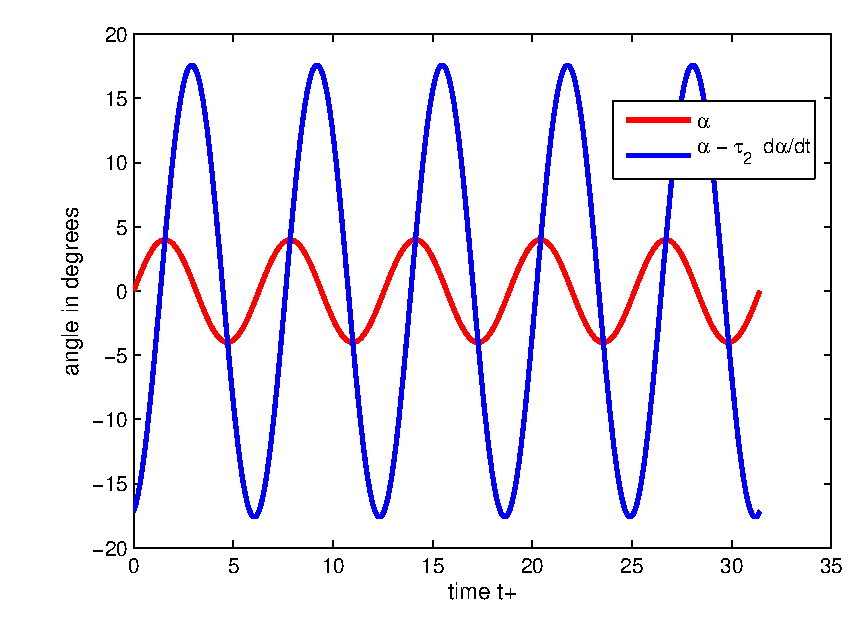
\includegraphics{./Figures/alpha_dalpha_sin_amp=4_k=0p5.eps}
  \caption{Effects of $\tau_2 \dot{\alpha}$ for high pitching rate}
  \label{fig:alpha_dalpha_vs_t}
\end{figure}


\begin{figure}[h]
  \centering
  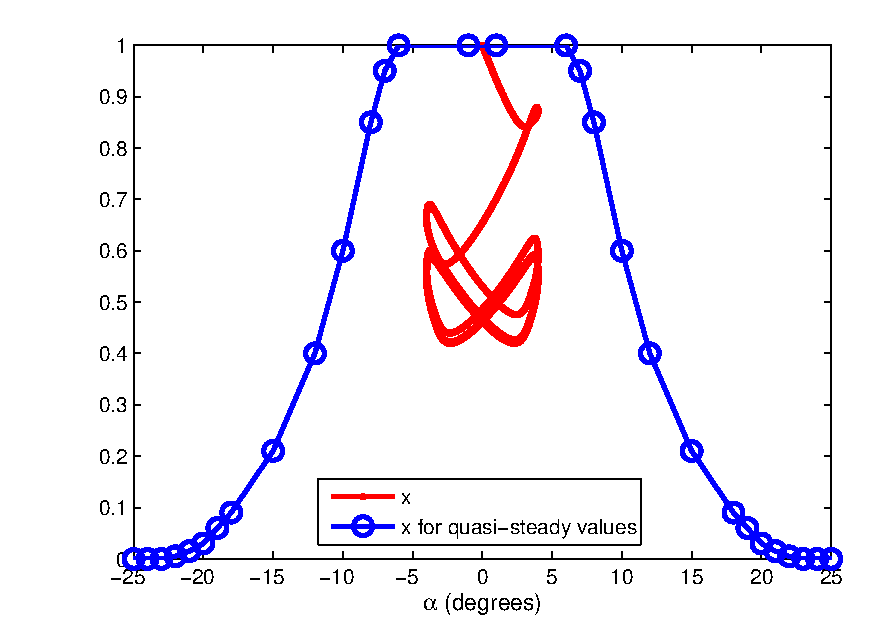
\includegraphics{./Figures/x_sin_amp=4_k=0p5.eps}
  \caption{State variable during fast sinusoidal pitching}
  \label{fig:x_fast_pitching}
\end{figure}

\par The state variable value starts at the quasi-steady value (as designed in the algorithm implementation) but after a couple of cycles it orbits close to an average value that would correspond to separated flows in a quasi-steady case.
This also leads to lower lift overall (see figure \ref{fig:Cl_fast_pitching}) since the value of x is smaller.

\begin{figure}[h]
  \centering
  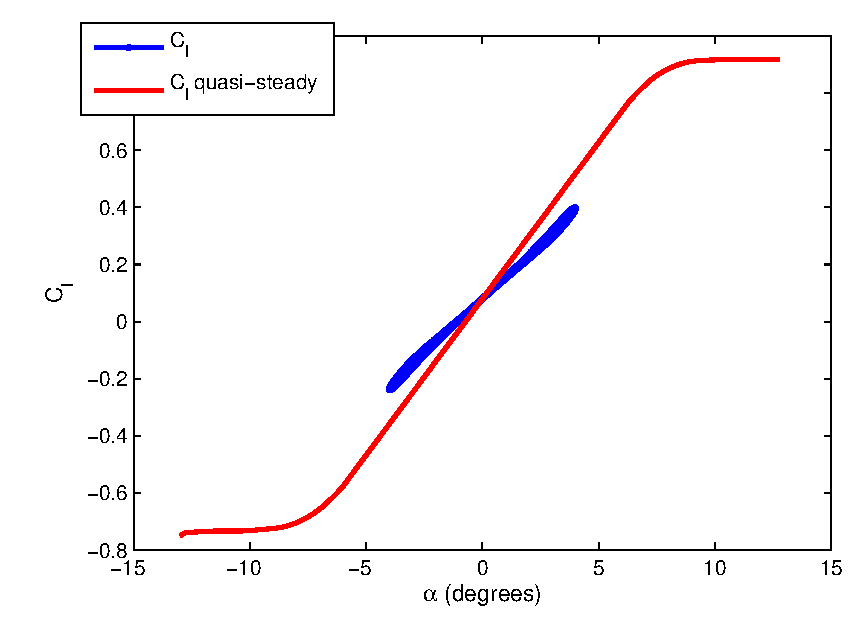
\includegraphics{./Figures/Cl_vs_alpha_amp=4_k=0p5.eps}
  \caption{$C_l$ is decreased compared to quasi-steady values for high pitching rate maneuvers (the transient part has been removed for clarity)}
  \label{fig:Cl_fast_pitching}
\end{figure}



\par If the exact same constraints are used for optimization the problem illustrated by figure \ref{fig:unlimited_alpha_dot}.	

\begin{figure}[h]
  \begin{center}
  
<++>%\includegraphics{<+file+>}
\end{center}
  \caption{Optimization for vertical wind gusts with the same constraints as the previous cases}
  \label{fig:unlimited_alpha_dot}
\end{figure}

The issue is that the in order to reach the favorable high lift regions the algorithm produces a 
%Since the lift to drag ratio of the NACA0009 is about 10 (compared to 13 for the notional UAV) direct comparisons with the results presented in part \ref{sec:results_QS} are impossible.
\Subsection{The ``staircase'' optimization issue}

All these effects dependent on the pitch rate add a lot of complexity to the optimization problem.
One of the biggest is that to keep a reasonably low execution time for the optimization the number of points has to be kept relatively low (less than a hundred).
Such discretization of the interval can cause issues in the discreet integration parts of the algorithm.
It seems that for most optimization cases this effect is avoided.

\par However the results of the of optimization for short gusts ($0.2<T_g<0.5$) sometime shows a ``staircase'' pattern in the angle of attack.

\begin{figure}[h]
  \centering
  %\includegraphics{<+file+>}
  \caption{Staircase pattern seen for XXXX wind gust with $T_g=XX$}
  \label{fig:staircase_case}
\end{figure}

\par In those cases the algorithm seems to try to ``game'' the GK model with this jerky pitch motion.
Our theory is that this jerky motion avoids the decrease of the lift coefficient caused by high pitch rates by doing those for only short amount of time.
These spikes in the pitch rate are too short to be able to influence the low pass equation regulating the value of $x$.





\Section{A closer look at the high performing short gusts}

\begin{figure}[h]
  \begin{center}
  \scalebox{0.4}{
    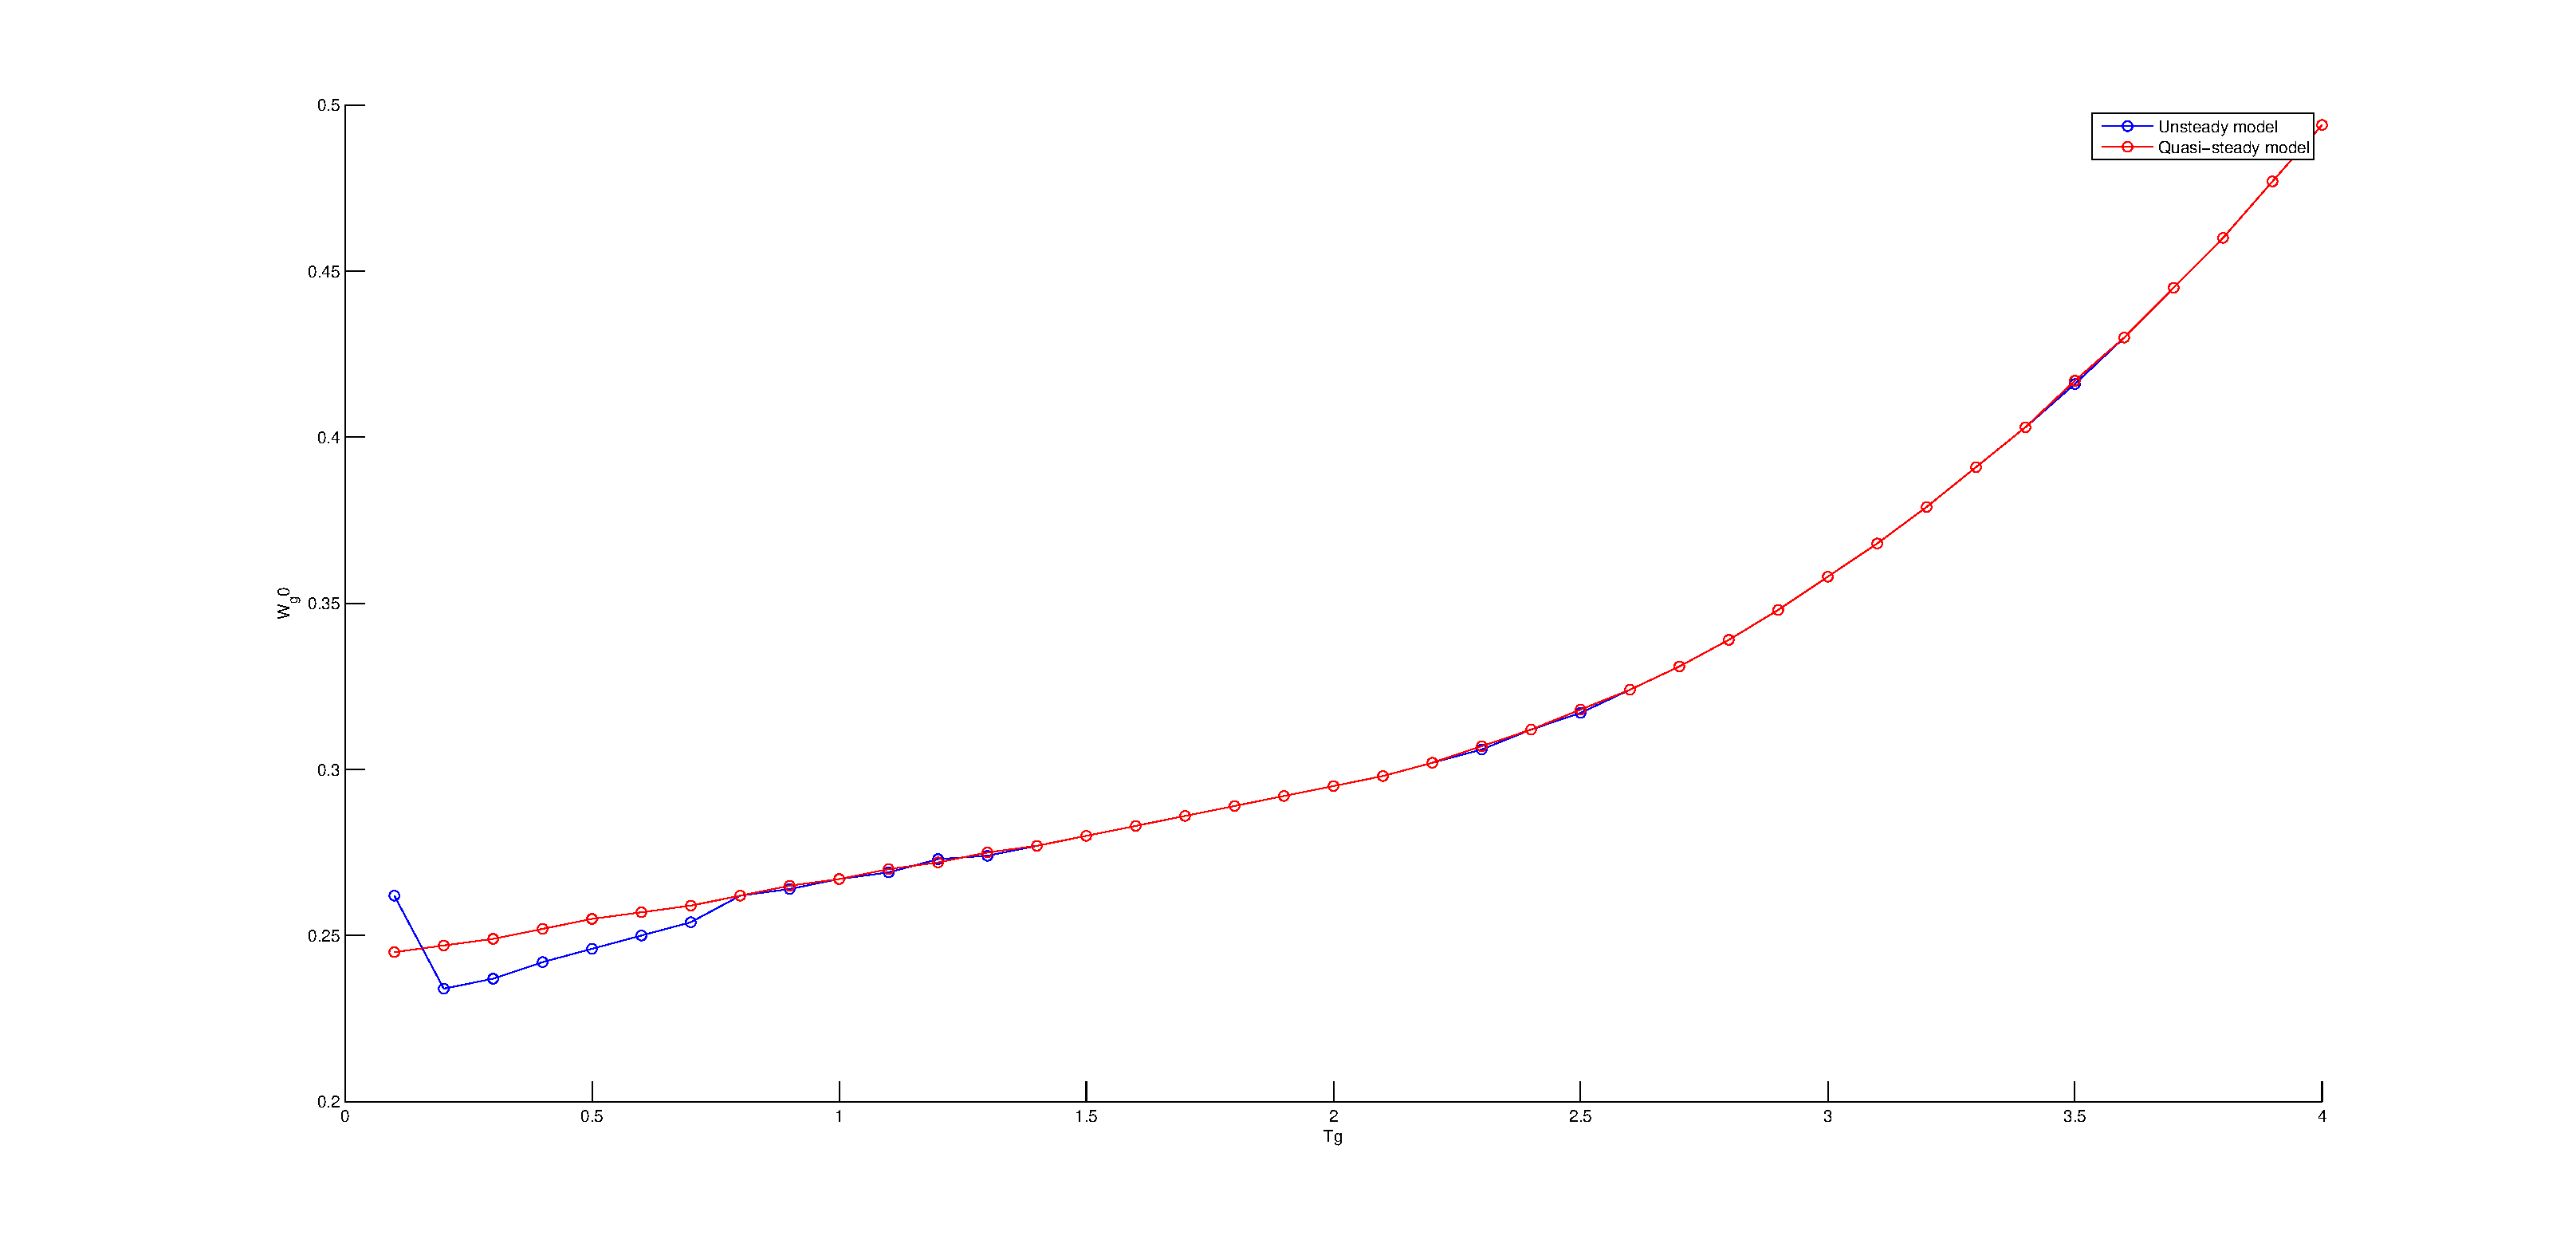
\includegraphics{./Figures/Wg_vs_TG_windtype=3_alphamax=12_nodalphalimit.eps}}
  \end{center}
  \caption{Performance difference between quasi-steady and unsteady model for combined gusts}
  \label{fig:WG_vs_TG_wt=3}
\end{figure}


\begin{figure}[h]
  \centering
  \scalebox{0.4}{
    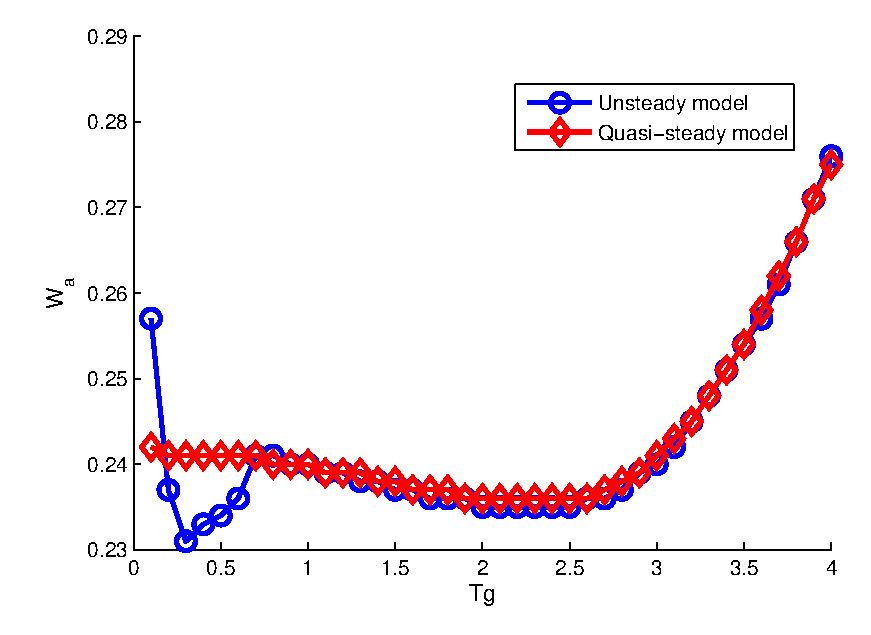
\includegraphics{./Figures/Wg_vs_TG_windtype=1_alphamax=12_nodalphalimit.eps}}
  \caption{Performance difference between quasi-steady and unsteady model for vertical gusts}
  \label{fig:WG_vs_TG_wt=1}
\end{figure}

\par The difference between the quasi-steady model and the unsteady one only appears close for $Tg<0.7$.
This result is reassuring as it confirm that for long gusts ($Tg>0.7$ or $k<0.05$) the two model are equivalent.
We can confirm that there is no unsteady effects active by looking at the $C_l$ versus $\alpha$ curve compared to the quasi-steady map, or even better $G$ the lift to drag ratio.
On figure \ref{fig:G_vs_alpha_wt=1_Tg=1_GK.eps} you can see that the lift to drag ratio for $T_g=1$ is following the quasi-steady values.

\begin{figure}[h]
  \centering
  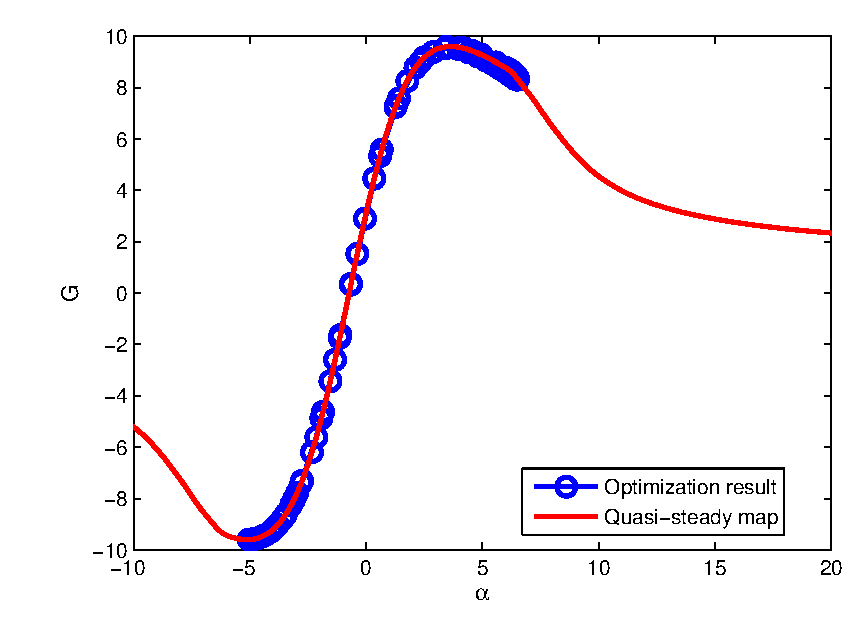
\includegraphics{./Figures/G_vs_alpha_wt=1_Tg=1_GK.eps}
  \caption{Lift to drag ratio for the unsteady model, vertical wind gust and gust duration of 1T}
  \label{fig:G_vs_alpha_wt=1_Tg=1_GK.eps}
\end{figure}

\par However for shorter gusts the results are more interesting.
We can see that for shorter gusts ($T_g<0.7$) the performances are better with the GK model than with the quasi-steady model.
This is true for both vertical and combined wind gusts which seems to indicate that this is due to the unsteady effects starting to be significant at this frequency.

\FloatBarrier

\par Looking more precisely at the results around $T_G=0.3$ let's try to highlight thee differences between the quasi-steady and the unsteady model.
First we can look at the optimization parameter $\alpha$ for both vertical and combined gusts.

\begin{figure}[h]
  \centering
  \scalebox{0.4}{
    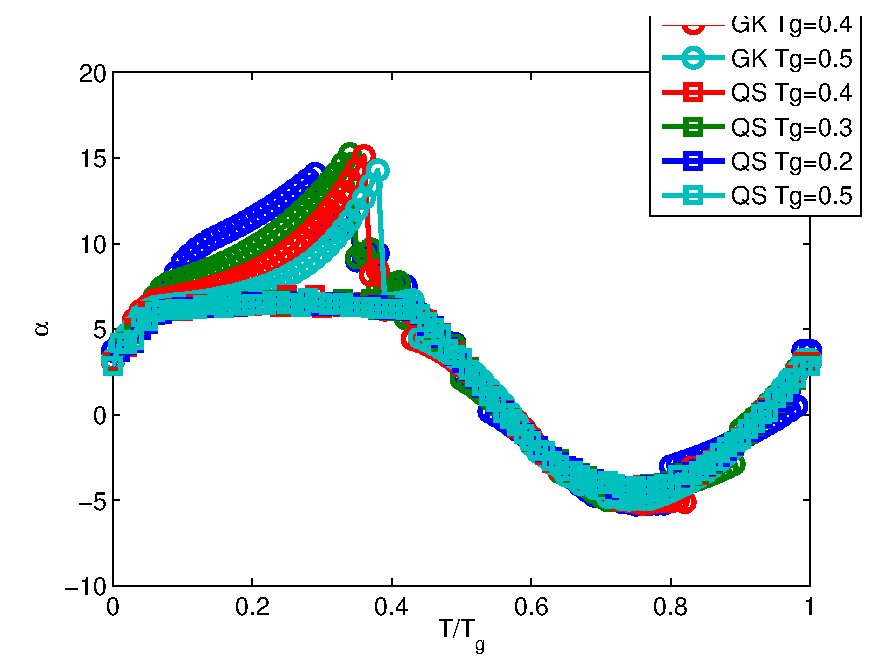
\includegraphics{./Figures/alpha_vs_Tg_wt1.eps}}
  \caption{Angle of attack for short vertical gusts with the quasi-steady (QS) and unsteady (GK) model}
  \label{fig:alpha_vs_Tg_wt1}
\end{figure}

\begin{figure}[h]
  \centering
  \scalebox{0.4}{
    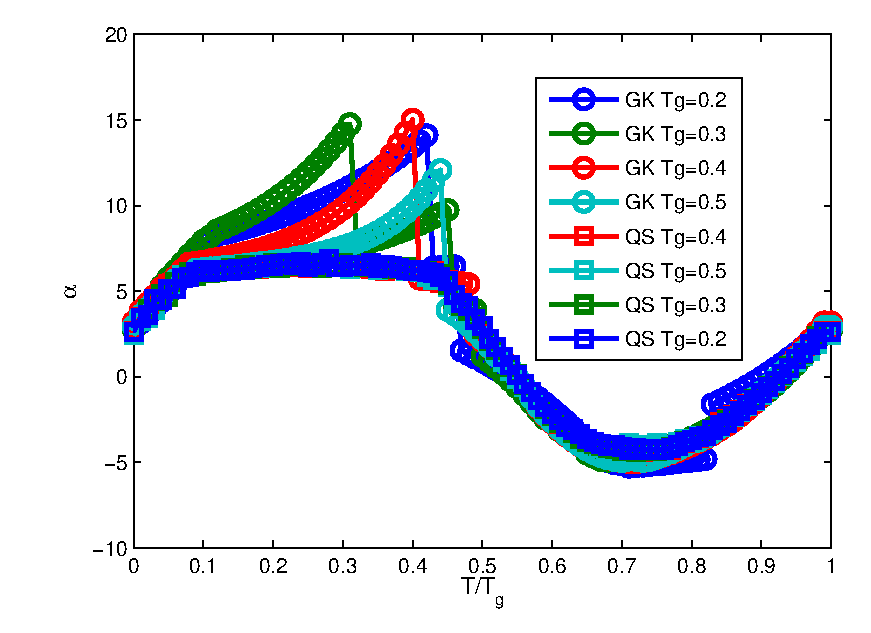
\includegraphics{./Figures/alpha_vs_Tg_wt3.eps}}
  \caption{Angle of attack for short combined gusts with the quasi-steady (QS) and unsteady (GK) model}
  \label{fig:alpha_vs_Tg_wt3}
\end{figure}

\par It is immediately apparent that the main difference is in the high angle of attack area.
Alpha increases exponentially before a sharp decrease happens around 30 to 40\% of the gust duration.
The angle of attack then falls back to the quasi-steady values.

\FloatBarrier

\par To understand what happens to the lift when such a maneuver is performed we have to refer to the lift coefficient versus angle of attack plot.

\begin{figure}[h]
  \centering
  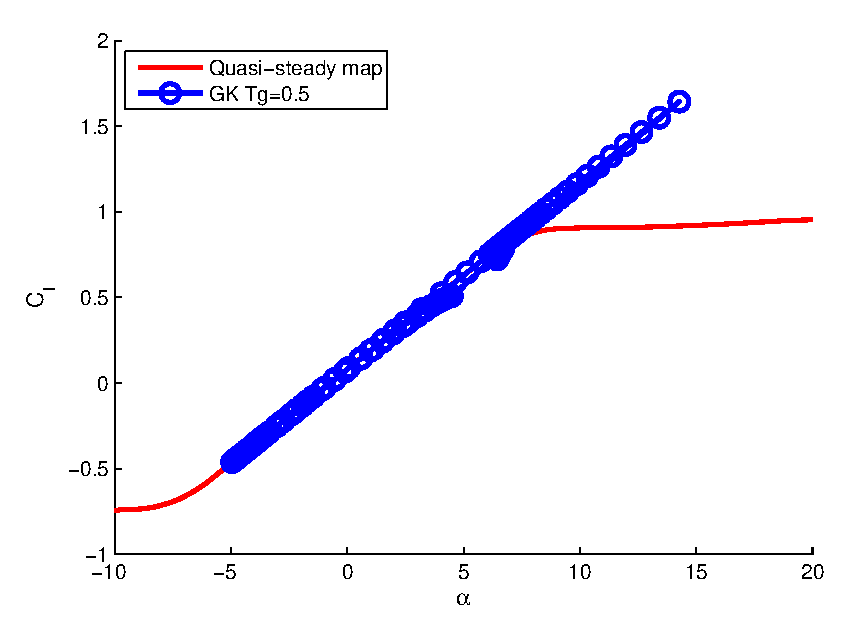
\includegraphics{./Figures/Cl_vs_alpha_wt=1_tg=0p5_alphamax=20.eps}
  \caption{Lift coefficient versus angle of attack for 0.5T long vertical wind gusts with the unsteady model}
  \label{fig:Cl_vs_alpha_short_gust_unsteady}
\end{figure}
\FloatBarrier

\par Figure \ref{fig:Cl_vs_alpha_short_gust_unsteady} illustrate perfectly the effects of the unsteady aerodynamic model and the difference with the quasi-steady model.
The spiking in angle of attack allows the flow to remain attached to the airfoil and let the lift coefficient reach values for superior to what the quasi-steady (red curve) model would ever permit.
Sharply decreasing the angle of attack at the end of this maneuver means that the flow doesn't have time to separate.
Similar results are observed for vertical and horizontal gusts in the $T_g=0.2$ to $0.7$ region.



\Section{Bad performances at $T_g\leq0.1$}

\par As seen on figures \ref{fig:WG_vs_TG_wt=3} and \ref{fig:WG_vs_TG_wt=1} while the unsteady model optimizations are showing a more efficient energy extraction than the quasi-steady for $0.2 \leq T_g \leq 0.7$ it is not the case at $T_g=0.1$. 


\Section{Limitations of the unsteady GK model}

\Subsection{Considering the gusting and plunging component}

One of the major thing this optimization misses are the unsteady effects due to gusting and plunging.
In our case we have major gusts present at the same time as the pitching motion.
While the speed of the UAV changes too, the relative wind amplitude is in the order of 20\%.
We know that gusts as gentle as 5\% of the free stream speed can have huge influence on the lift characteristics and that the lift response to such gusts depends heavily on the frequency of the gusts.
The same can be said for the plunging motion.

\par While this variations are pretty wild it is suspected that they are caused by the same kind of mechanism as the lift variations caused by pitch angle changes.
With that in mind there is a fairly high probability that the resulting mechanism could be described by a model inspired by the GK model.
It is very likely that the state variable for such a model would be tied in some way to the state variable presented in this thesis.
If $x$ could be expressed as a function of $\alpha$, $\dot{\alpha}$ and $\dot{u}$ (for example), this model could be applicable to a whole new range of situations.



\Subsection{Moment of inertia considerations}



\Chapter{CONCLUSION}

\Section{Low order model for unsteady flow}

\par The Goman and Khrabrov model shows good agreement in both shape and magnitude for the lift and drag of a pitching airfoil in a wide range of conditions.
It is fast and light and can be adjusted to a new airfoil (or even a whole aircraft) without requiring extensive experimental studies.
In fact in theory only a static map and one unsteady case should be enough to obtain the whole model.

\par The work in this thesis has proven that the drag can also be easily modeled and there is little doubt that the moment coefficient $C_m$ could be modeled too.

\par Implementing this model is simple enough that it can be used in computationally heavy applications such as optimization problems or real time applications.
It is however non-linear and as such isn't easily invertible or analyzable with traditional control system methods.

\Section{Energy extraction optimization}

\par From the results presented in this thesis it can be seen that energy extraction can be performed for complex temporal wind gusts with vertical and horizontal components.
In these gusts overall neutral energy trajectories are possible and require less and less wind gust amplitude the shorter the gust is.
For short gust ($T_g \le 3$) high angles of attack are needed for maximum performance, which can lead to flow separation.

\par The introduction of an unsteady aerodynamic model is possible and proves necessary when gusts are very short ($T_g \le 0.7$ or $k \ge 0.05)$).
At this point unsteady effects such as lag in the flow separation can be observed and even taken advantage of.
While the maneuvers required to obtain such trajectories are unlikely to be realistically done on aircrafts, these results could be exploited in vertical wind turbine pitch optimization for example.
The results for gusts shorter than $T_g=0.2$ ($k=0.175$) are less obvious to interpret and will require further study, perhaps with a problem more representative of the system operating at such frequencies.

\par While these results shows the optimal trajectory found by the algorithm it is important to keep in mind that the algorithm optimize the trajectory globally over the whole period.
This means that it can take preemptive actions because it ``knows'' what will happen later in time.
A real controller flying in an environment where the wind gust shape can't be predicted would not be able to reach the same energy extraction performances.

\Section{Possible improvements and additional work}

\par One of the weakness of the optimization with the GK model is that it does not account for the unsteady effects due to the surging and gusting components of the relative wind.
I believe that the GK model could be modified to include these effects but a complete experimental campaign would be needed.

\par The ``staircase'' effect described in section \ref{sub:staircase} could be mitigated by introducing a more realistic model for the aircraft dynamics that include the moment of inertia.
Going even further, a basic elevator model could be implemented.

\par Finally replacing the temporal wind profile by a spatial one would allow for the use of more realistic and complex wind fields.




\clearpage


%
% APPENDIX
%

% Do the settings of appendices with \appendix command
\appendix

% Then create each appendix using
% \Appendix{title_of_appendix} command

\Appendix{Goman Khrabrov model Matlab\textsuperscript{\textregistered} implementation} \label{ch:GK_code}
\lstinputlisting{./NACA0009_GK.m}
%\moretox




%
% BIBLIOGRAPHY
%
% you have two options: 1) create bibliography manually,
% 2) create bibliography automatically. See BibliographyHelp.pdf file for details.


\bibliographystyle{plain}
\bibliography{mybib}


\end{document}  % end of document
